%% ##############################################################################################
%% Plantilla estandar para el documento de tesis para la maestri�a en ciencias computacionales
%% en la UAG.
%% Fecha ultima modificacion: 04 de agosto de 2018
%% Editada por: Efrain Adrian Luna Nevarez
%% ##############################################################################################

\documentclass[12pt,letterpaper,spanish]{book}
%\spanishdecimal{.}

% Encabezados y pies de pagina
\usepackage{fancyhdr}

% para usar de manera natural los acentos, tildes y �, ademas del respectivo diccionario de espa�ol
%\usepackage[utf8]{inputenc}
\usepackage[latin1]{inputenc}
\usepackage[spanish,activeacute]{babel}
\usepackage{musixtex}
\spanishdecimal{.}
\usepackage{amsmath}
\usepackage{amssymb}
\usepackage{amsthm}
\usepackage{algorithmic}
\usepackage{algorithm}
\usepackage{cool} %Sumatorias cool

% para tablas largas
\usepackage{longtable}
\usepackage{array}

% para incluir los apendices
\usepackage{appendix}

% para incluir graficas y subgraficas dentro de las gr�ficas etc., etc.
\usepackage{graphicx}
\usepackage{subfigure}
\usepackage{wrapfig}
\usepackage{float}
\usepackage{caption}
%\usepackage{subcaption}
\graphicspath{{imagenes/}}

%\usepackage{subfig}%%%%%
%\usepackage{float}   %%%%% tambien nuevo
%\usepackage[hKV-listi]{subfig} %%%% nuevo

% para definir algunos margenes personalizados
\usepackage{anysize}
\marginsize{1.5in}{1in}{1in}{1in}
\usepackage[nottoc]{tocbibind}
\usepackage{setspace}

% para tablas con celdas compartidas
\usepackage{multirow}
\usepackage{fancybox}
\usepackage{bigstrut}
\usepackage{booktabs}


% para incluir colores en texto o en celdas de las tablas
\usepackage{color}
\usepackage{colortbl}

% para el estilo natbib de bibliografi�as (sino lo usan no va)
\usepackage{cite}

\usepackage{titlesec}

% para incluir paginas de un archivo pdf
\usepackage{pdfpages}

%##############################################################################
% para renombrar algunos ti�tulos
\renewcommand{\appendixname}{Apendices}
\renewcommand{\appendixtocname}{Apendices}
\renewcommand{\appendixpagename}{Apendices}

%##############################################################################
% incluimos informacion personalizada para algunos valores de la plantilla
\newcommand{\tstamp}{\small [\thepage]}
\newcommand{\Escuela}{\scshape \scriptsize}
\newcommand{\Uni}{\scshape \scriptsize Universidad Aut�noma de Guadalajara}
\newcommand{\TEMA}{\scshape \scriptsize ``Uso de Deep Learning para composici�n musical''}


%##############################################################################
% redefinimos los espacios para las figuras

\newcommand{\figura}[5]{
  \begin{figure}[#5]
  \begin{center}
  \includegraphics[#2]{#1}
  \caption[#3]{#3}
  \label{#4}
  \end{center}
  \end{figure}
}
%##############################################################################
% redefinimos los espacios para las tablas
\newenvironment{tabla}[2]{
  \begin{table}[#2]
  \begin{center}
  \caption[#1]{#1}
}{
  \end{center}
  \end{table}
}

%##############################################################################
% renombramos algunas constantes para entornos matematicos
\def\sen{{\rm sen \ }}
\def\cos{{\rm cos \ }}

\def\a{\mathbf a}
\def\b{\mathbf b}
\def\c{\mathbf c}
\def\d{\mathbf d}
\def\e{\mathbf e}
\def\ex{\mathrm e}
\def\f{\mathbf f}
\def\g{\mathbf g}
\def\h{\mathbf h}
\def\k{\mathbf k}
\def\n{\mathbf n}
\def\m{\mathbf m}
\def\p{\mathbf p}
\def\q{\mathbf q}
\def\P{\mathbf P}
\def\R{\mathbf R}
\def\T{\mathbf T}
\def\L{\mathbf L}
\def\r{\mathbf r}
\def\u{\mathbf u}
\def\v{\mathbf v}
\def\w{\mathbf w}
\def\x{\mathbf x}
\def\y{\mathbf y}
\def\z{\mathbf z}
\def\sen{{\rm sen \ }}

%################################################################################
% rebombramos las etiquetas para retuilizar la informaci�n antes ingresada
\renewcommand{\labelenumi}{\textbf{\theenumi}.-}
\renewcommand{\labelenumii}{\textbf{\theenumi}.-}
\renewcommand{\labelenumiii}{\textbf{\theenumi}.-}
\renewcommand{\labelenumiv}{\textbf{\theenumi}.-}



%#################################################################################
% especificamos casos extraodinarios para la divisi�n de palabras
\hyphenation{es-pe-cia-li-dad} \hyphenation{ob-te-ner}
\hyphenation{des-ple-gar}
\hyphenation{original}
\hyphenation{geo-gra-fi-ca} \hyphenation{do-cu-men-to}
\hyphenation{do-cu-men-tos}
\hyphenation{e-va-lua-da}\hyphenation{pro-pues-ta}
\hyphenation{tu-ris-mo}\hyphenation{pro-pues-to}
\hyphenation{ma-yo-res}\hyphenation{des-cri-be}
\hyphenation{re-le-van-cia}\hyphenation{pro-ble-ma}
\hyphenation{ma-ne-ra}\hyphenation{co-rres-pon-de}
\hyphenation{pro-pues-to}\hyphenation{re-tro-a-li-men-ta-cion}
\hyphenation{si-mi-li-tud}\hyphenation{tradicional}\hyphenation{ordenamiento}
\hyphenation{pu-bli-ca-cio-nes}\hyphenation{a-tri-bu-tos}
\hyphenation{re-cu-pe-rar}\hyphenation{re-cu-pe-ra-das}

% espaciado : 1 y 1/2
\onehalfspacing

% establecemos la enumeraci�n para las equaciones y figuras
\numberwithin{equation}{section}
\renewcommand{\thefigure}{\thechapter.\arabic{figure}}

\setlength{\arrayrulewidth}{1pt}
\setlength{\doublerulesep}{0mm}

\sloppy
\frenchspacing

% redefinimos el comando para incrustar dos p�ginas vac��as
\newcommand{\clearemptydoublepage}{\newpage{\pagestyle{empty}\cleardoublepage}}


%#################################################################################
% inicio del documento
\begin{document}

% incluimos el pdf con la portada como primera p�gina de este documento
% nota: debes modificar y compilar de manera separada el archivo portada.tex, luego compilar este documento para que incluya la versi�n modificada del PDF (portada.pdf)
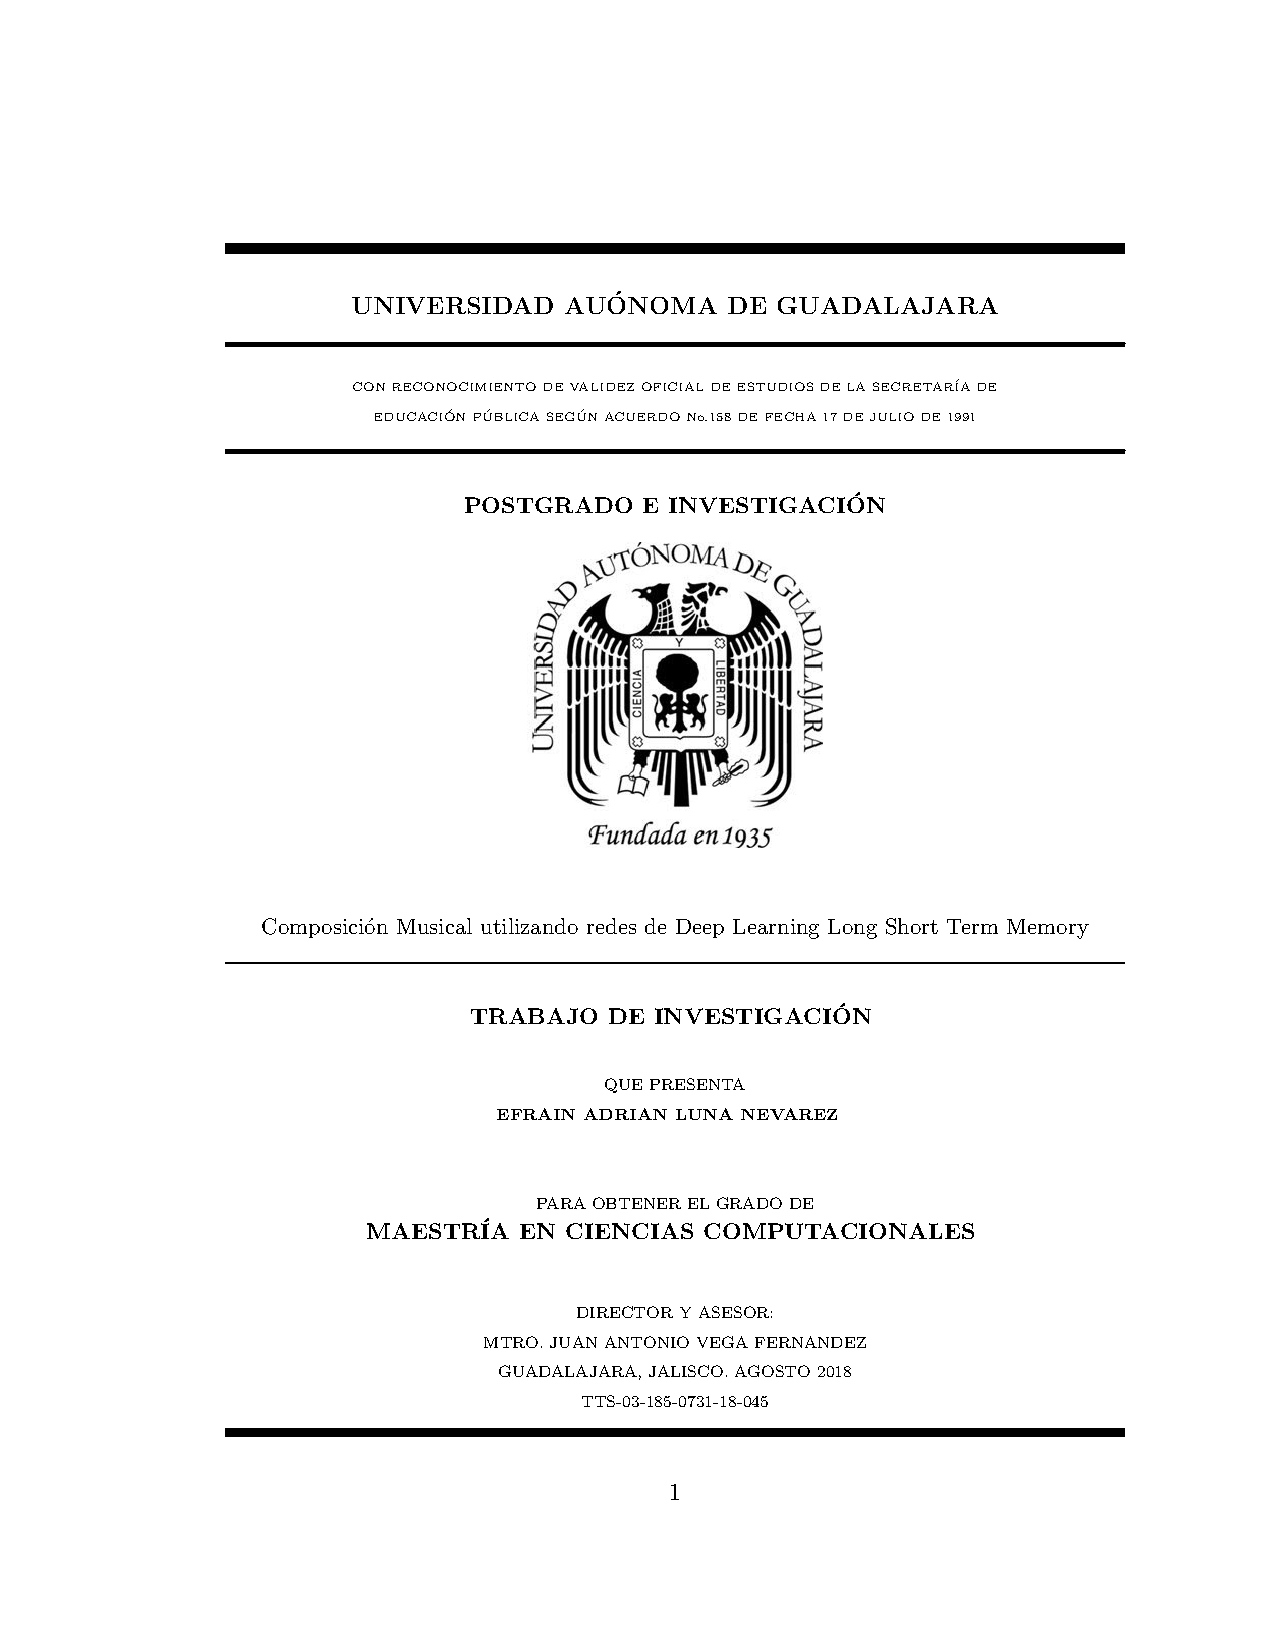
\includepdf[pages=1]{portada.pdf}
\clearemptydoublepage

% incluimos el .tex que tiene la informaci�n para la contraportada (puede llamarse como desees, pero recuerda poner el nombre sin extensi�n)
\include{contraportada}                  %%%%%%%%
\clearemptydoublepage


\frontmatter
\pagestyle{fancyplain}



%###############################################################################33
% redefinimos los m�rgenes para el documento
\setlength{\topmargin}{0.0cm}
\setlength{\headsep}{0.5cm}
\setlength{\headheight}{0.5cm}

\setlength{\marginparsep}{0mm}
\setlength{\marginparwidth}{0cm}

\setlength{\footskip}{1.5cm}

  \setlength\paperheight {11in}
  \setlength\paperwidth  {8.5in}

  \setlength{\textwidth}{6in}
  \setlength{\textheight}{8.5in}

  \setlength{\marginparwidth}{0cm}
  \setlength{\voffset}{0.0in}
  \setlength{\hoffset}{0.0in}

 %\setlength{\evensidemargin}{0.32} % margen paro lvera
  \setlength{\evensidemargin}{0in} % margen par
  \setlength{\oddsidemargin}{0.32in}  % margen impar
 % \setlength{\oddsidemargin}{0in}  % margen impar



%###################################################################################
% especificamos el nombre en espa�ol para cada secci�n est�ndar de la tesis
\def\contentsname{\'{I}ndice General}
\def\contentsname{Tabla de Contenido}
\def\listfigurename{Lista de Figuras}
\def\listtablename{Lista de Tablas}
\def\bibname{Bibliograf�a}
\def\indexname{\'{I}ndice Alfabetico}
\def\figurename{\bf \scriptsize Figura}
\def\tablename{\bf \scriptsize Tabla}
\def\partname{Parte}
\def\chaptername{Cap\'{i}tulo~\thechapter}
\def\appendixname{Ap\'{e}ndice}
\def\abstractname{Resumen}

% presentaci�n de titulo y capitulo
\renewcommand{\chaptermark}[1]{\markboth{#1}{}}
% Numero y titulo de seccion
\renewcommand{\sectionmark}[1]{\markright{\thesection~~ #1}}


\lhead[\fancyplain{}{\small \thepage}]{\fancyplain{}{\scshape
\scriptsize \rightmark}} %\rightmark = información sobre el capítulo

\rhead[\fancyplain{}{\scshape \scriptsize
\leftmark}]{\fancyplain{}{\small \thepage}} %\leftmark = información sobre la sección

\lfoot[\fancyplain{}{\Escuela}]{\fancyplain{}{}}
\cfoot[\fancyplain{\tstamp}{}]{\fancyplain{\tstamp}{\TEMA}}
\rfoot[\fancyplain{}{\Uni}]{\fancyplain{}{}}

\renewcommand{\headrulewidth}{0.4pt}
\renewcommand{\footrulewidth}{\headrulewidth}

% cambiar el formato para los ti�tulos
\newcommand{\bigrule}{\titlerule[0.5mm]}

\titleformat{\chapter}[display]
{\bfseries \Huge } {
 \titlerule
 \filleft\Large\chaptertitlename
 }
{0mm} {\filleft}
 [\vspace{0.5mm}\bigrule]

%###################################################################################

% incluimos los .tex de cada uno de las secciones previas al verdadero documento.
% los puntos .tex van sin preambulo, instrucciones para definir ti�tulo, secciones, subsecciones, tablas, etc.
%IMD PNA http://na.support.keysight.com/pna/help/latest/Applications/Swept_IMD_Configure_External_Source_and_Combiner.htm

\vspace*{\fill}
\begin{center}
	\textbf{\huge Dedicatoria}
\end{center}

\begin{center}
Este trabajo se lo dedico a todos los m�sicos que sean apasionados por la tecnolog�a, y ven en ella una forma para seguir evolucionando musicalmente. 
\end{center}
\vspace*{\fill}

%%-----------------------------------------------------------------------


%IMD PNA http://na.support.keysight.com/pna/help/latest/Applications/Swept_IMD_Configure_External_Source_and_Combiner.htm
\begin{center}
\textbf{\huge Agradecimientos}
\end{center}

Primeramente agradezco a Dios por permitirme haber concluido un ciclo mas en mi formaci�n profesional, cada paso que doy siempre es gracias a �l.

Agradezco a mi madre por ense�arme el valor del trabajo y del estudio. Gracias a ella que me brindo un consejo cuando lo necesite, un hombro de apoyo cuando flaqueaba y una reprimenda cuando no estaba asciendo las cosas correctamente.

A mi novia que estuvo conmigo en �pocas dif�ciles en mi vida, cuando pens� que no podr�a terminar con mis estudios por todas las responsabilidades que hab�a adquirido, ella siempre estuvo ah� para animarme a seguir adelante.

Mis hermanas las cuales siempre me dieron palabras de aliento y estuvieron preocupadas por mi, en todo momento, agradezco su apoyo incondicional.

Al CONACYT porque me brindo el apoyo econ�mico para poder terminar este grado de estudio.

A mis maestros que tuvieron la suficiente paciencia y dedicaci�n para transmitirnos parte de su conocimiento, gracias a ellos pude concluir con este grado, ganando el suficiente conocimiento para poder aplicarlo en el campo laboral.

A mi Asesor el Maestro Juan Antonio Vega Fern�ndez, el cual me gu�o a lo largo de esta tesis para realizar un trabajo que pueda dejar algo de conocimiento a la comunidad, agradezco la paciencia que me tuvo y el tiempo que me dedico para la revisi�n de este proyecto.

A mis compa�eros de generaci�n los cuales me ense�aron much�simas cosas, fue muy enriquecedor contar con personas que a pesar de que hab�an vivido cosas muy diferentes, ten�an en la mente seguir super�ndose escolarmente y profesionalmente hablando.

Finalmente agradezco a la UAG, escuela que me dejo tanto aprendizaje y vivencias. A todo el personal administrativo de esta instituci�n que me guiaron a trav�s de todos los tramites necesarios para concluir esta etapa.

%%-----------------------------------------------------------------------


%IMD PNA http://na.support.keysight.com/pna/help/latest/Applications/Swept_IMD_Configure_External_Source_and_Combiner.htm
\begin{center}
\textbf{\huge Resumen}
\end{center}

En este trabajo, se analizaron diferentes tipos de arquitecturas de redes de Deep Learning, con el fin de usarlas para crear nuevas piezas musicales.

Estas redes usan capas de neuronas Long Short Term Memory (LSTM), las cuales nos permitieron trabajar con secuencias de datos y guardar informaci�n a lo largo del tiempo.

Las redes descritas en este proyecto fueron entrenadas para reconocer y generar secuencias para los instrumentos de guitarra y bajo el�ctrico.

El proceso de entrenamiento se logro usando una base de datos de archivos MIDI, los cuales son de genero rock y pop, por lo tanto, el aprendizaje de estas redes �nicamente sera para reconocer estos g�neros musicales.

Las arquitecturas usadas fueron entrenadas para reconocer tonalidades de las canciones y en base a ellas generar nuevas piezas musicales.

%%-----------------------------------------------------------------------


\include{abstracto}


% por si quieres incuir hasta un tercer nivel en la tabla de contenidos
%\setcounter{tocdepth}{3}

% creamos la tabla de contenidos y las listas de figuras y tablas
\tableofcontents         %%
\listoffigures           %%
\listoftables            %%

\mainmatter
\renewcommand{\chaptermark}[1]{\markboth{\thechapter.~~#1}{}}

%########################################################################################
% ahora si incluimos cada uno  de los .tex correspondientes a los capitulos de la tesis. Es mas claro dividir los capitulos en .tex aunque puedes poner todo el texto aqui�.
% los puntos .tex van sin preambulo, es decir que va el texto correspondiente y las instrucciones para definir titulo, secciones, subsecciones, tablas, etc.

\chapter{Introducci�n}

La m�sica es el idioma universal, no importa en qu� lugar f�sico nos encontremos, todos alguna vez hemos escuchado una canci�n que se nos queda grabada en la cabeza por mucho tiempo. En ocasiones nos preguntamos c�mo es que el autor compuso esa canci�n.

Existen muchos g�neros musicales, cada uno cuenta con sus propias reglas, ritmos y sonidos caracter�sticos, por lo que los compositores que se dedican a crear nuevas canciones para cada genero en especifico, deben de tener una gran noci�n acerca del mismo asi como sus generalidades. Es por eso que nos ponemos a pensar si una computadora es capaz aprender a reconocer las generalidades de un genero musical y generar nuevas piezas musicales en base a esto.

Si bien es cierto el componer una canci�n es un arte, las canciones se pueden interpretar en forma matem�tica, esto nos abre la posibilidad de usar algoritmos computacionales para la creaci�n de nuevas canciones.

\section{Descripci�n del Problema}

Los principales problemas en la composici�n musical son: la falta de ideas y el tiempo requerido para la composici�n.

Existen compositores que a lo largo del tiempo no les gusta explorar nuevas formas o ritmos musicales y eso ocasiona que sus composiciones sean muy similares entre si.

El tiempo requerido para la creaci�n de una nueva canci�n es muy variado, ya que depende del g�nero, el n�mero de instrumentos y la complejidad de la composici�n. 

En este trabajo se busca usar un algoritmo computacional, que nos permita generar nuevas canciones de una manera m�s r�pida y sencilla.

\section{Objetivos}
\subsection{Objetivo General}

Creaci�n de un programa que use algoritmos para servir de apoyo para composici�n musical.

\subsection{Objetivos Espec�ficos}
\begin{enumerate}
  \item Implementar una red neuronal de Deep Learning que sea capaz de crear melod�as y armon�as musicales en guitarra.
  \item Implementar una red neuronal de Deep Learning que sea capaz de crear melod�as musicales en bajo el�ctrico.
  \item Conjuntar la salida de las redes neuronales para generar un solo archivo de audio.
  \item Verificar la Tonalidad de la canci�n resultante.
  \item Comparar las diferentes arquitecturas.
\end{enumerate}

\section{Justificaci�n}

El uso de algoritmos de Deep Learning en la m�sica no es algo nuevo, sin embargo, existen muchas �reas de oportunidad en cuesti�n de la implementaci�n de estos algoritmos.

En el articulo ''Deep Learning Techniques for Music Generation - A Survey'' \cite{DBLP:journals/corr/abs-1709-01620} podemos observar diferentes maneras para crear m�sica con redes neuronales de Deep Learning. Este es uno de los trabajos mas completos que existen hasta la fecha. Los autores de este articulo comparan diferentes estilos de redes (CNN, RNN y generativas), para ver cual es la que mejor para creaci�n musical. Aunque es un articulo muy completo no se aborda como hacer que las redes aprendan a distinguir tonalidades.

El articulo ''Deep Learning for Music'' \cite{DBLP:journals/corr/HuangW16} presenta una buena forma para la creaci�n de armon�as y melod�as musicales utilizando redes de Deep Learning y archivos en formato MIDI. En este trabajo hacen falta maneras para validar la salida musical.

La mayor parte de los trabajos en esta �rea est�n basados en melod�as y armon�as de piano, sin embargo es interesante experimentar con otros instrumentos, ya que cada uno cuenta con su propia manera de interpretar una pieza musical.

Lo que se pretende en esta investigaci�n es tener una manera f�cil y r�pida para la creaci�n de nuevas composiciones musicales de guitarra y bajo.

\section{Delimitaci�n}

Este proyecto se centrara en crear melod�as y armon�as musicales de guitarra y bajo el�ctrico por lo que no se analizaran otros instrumentos.

Las nuevas canciones creadas por estos algoritmos no buscan ser ideas finales de composici�n, la �nica intensi�n es crear una serie de ideas para nuevas canciones.

La base de datos usada para entrenar a la red neuronal consta de canciones de genero rock y pop unicamente, no se entrenara la red para reconocer y generar canciones de otros g�neros musicales.

\section{Organizaci�n de la Tesis}

Esta tesis se divide en varios cap�tulos, los cuales se describen a continuaci�n.

\begin{itemize}
	\item \textbf{Capitulo 1.-} Se presenta una descripci�n del problema, justificaci�n, delimitaci�n y antecedentes hist�ricos de la investigaci�n.
	\item \textbf{Capitulo 2.-} Contiene el marco te�rico de las redes neuronales y su clasificaci�n. 
	\item \textbf{Capitulo 3.-} Aborda el marco te�rico musical, todos los conceptos b�sicos para interpretar y leer m�sica.
	\item \textbf{Capitulo 4.-} Se muestra el desarrollo del proyecto, la arquitectura y los componentes del sistema.
	\item \textbf{Capitulo 5.-} Contiene los resultados de las diferentes etapas del proyecto.
	\item \textbf{Capitulo 6.-} Se muestran las conclusiones del proyecto, as� como tambi�n los trabajos futuros que podr�an realizarse.
\end{itemize}

\section{Antecedentes hist�ricos}

A lo largo del tiempo han surgido varios estudios referentes al uso de algoritmos de Deep Learning con la m�sica, a continuaci�n se presentan algunos de los art�culos mas relevantes en este tema:

\subsection{Unsupervised Feature Learning for Audio Classification Using Convolutional Deep Belief Networks \cite{Lee:2009:UFL:2984093.2984217}}

''En los �ltimos a�os, los enfoques de Deep Learning han ganado un gran inter�s como una forma de construir representaciones jer�rquicas a partir de datos sin etiquetar. Sin embargo, seg�n nuestro conocimiento, estos enfoques de Deep Learning no se han estudiado exhaustivamente para datos auditivos. En este documento, aplicamos redes de creencias profundas convolucionales a los datos de audio y los evaluamos emp�ricamente en varias tareas de clasificaci�n de audio. Para el caso de datos de voz, mostramos que las caracter�sticas aprendidas corresponden a tel�fonos / fonemas. Adem�s, nuestras representaciones de funciones entrenadas a partir de datos de audio sin etiquetar muestran un rendimiento muy bueno para m�ltiples tareas de clasificaci�n de audio. Esperamos que este documento inspire m�s investigaci�n sobre los enfoques de aprendizaje profundo aplicados a una amplia gama de tareas de reconocimiento de audio.''

\subsection{Feature Learning and Deep Architectures: New Directions for Music Informatics \cite{Humphrey:2013:FLD:2590112.2590133}}

''A medida que buscamos avanzar en el estado del arte en inform�tica de m�sica basada en contenido, hay un sentido general de que el progreso se est� desacelerando en todo el campo. En una inspecci�n m�s cercana, las trayectorias de rendimiento en varias aplicaciones revelan que este es realmente el caso, lo que plantea algunas preguntas dif�ciles para la disciplina: �por qu� nos estamos desacelerando y qu� podemos hacer al respecto? Aqu�, nos esforzamos por abordar estas dos preocupaciones. Primero, revisamos cr�ticamente el enfoque est�ndar para el an�lisis de la se�al de m�sica e identificamos tres deficiencias espec�ficas de los m�todos actuales: el dise�o de caracter�sticas artesanal es sub�ptimo e insostenible, el poder de las arquitecturas poco profundas es fundamentalmente limitado y el an�lisis a corto plazo no puede codificar musicalmente estructura significativa Reconociendo los avances en otros dominios perceptivos de inteligencia artificial, ofrecemos que el aprendizaje profundo tiene el potencial de superar cada uno de estos obst�culos. A trav�s de argumentos conceptuales para el aprendizaje de caracter�sticas y arquitecturas de procesamiento m�s profundas, demostramos c�mo los modelos de procesamiento profundo son extensiones m�s poderosas de los m�todos actuales y por qu� ahora es el momento de este cambio de paradigma. Finalmente, concluimos con una discusi�n de los desaf�os actuales y el impacto potencial para motivar a�n m�s una exploraci�n de esta �rea de investigaci�n prometedora.''

\subsection{Improving Content-based and Hybrid Music Recommendation Using Deep Learning \cite{Wang:2014:ICH:2647868.2654940}}

''Los sistemas de recomendaci�n de m�sica basados ??en contenido existentes suelen emplear un enfoque \ textit {two-stage}. Primero extraen caracter�sticas de contenido de audio tradicionales como los coeficientes cepstral de frecuencia de Mel y luego predicen las preferencias del usuario. Sin embargo, estas caracter�sticas tradicionales, originalmente no creadas para la recomendaci�n de m�sica, no pueden capturar toda la informaci�n relevante en el audio y, por lo tanto, limitar el rendimiento de la recomendaci�n. Usando un modelo novedoso basado en una red de creencias profundas y un modelo gr�fico probabil�stico, unificamos las dos etapas en un proceso automatizado que aprende simult�neamente las caracter�sticas del contenido de audio y hace recomendaciones personalizadas. Comparado con los modelos basados en Deep Learning existentes, nuestro modelo supera a los de las etapas de arranque en caliente y de arranque en fr�o sin depender del filtrado colaborativo (CF). Luego presentamos un m�todo h�brido eficiente para integrar a la perfecci�n las caracter�sticas aprendidas autom�ticamente y la CF. Nuestro m�todo h�brido no solo mejora significativamente el rendimiento de la FQ, sino que tambi�n supera el m�todo h�brido basado en caracter�sticas tradicionales.''
\newpage

\subsection{Deep Learning for Music \cite{DBLP:journals/corr/HuangW16}}

''Nuestro objetivo es poder construir un modelo generativo a partir de una arquitectura de red neuronal profunda para intentar crear m�sica que tenga armon�a y melod�a y que sea pasable como m�sica compuesta por humanos. El trabajo anterior en la generaci�n de m�sica se ha centrado principalmente en crear una sola melod�a. El trabajo m�s reciente sobre el modelado de m�sica polif�nica, centrado alrededor de la estimaci�n de densidad de probabilidad de series de tiempo, ha logrado cierto �xito parcial. En particular, ha habido mucho trabajo basado en redes neuronales recurrentes combinadas con m�quinas de Boltzmann restringidas (RNN-RBM) y otros modelos similares basados en energ�a recurrente. Sin embargo, nuestro enfoque es realizar el aprendizaje y la generaci�n de extremo a extremo solo con redes neuronales profundas.''

\subsection{End-to-end learning for music audio tagging at scale \cite{DBLP:journals/corr/abs-1711-02520}}

''La falta de datos tiende a limitar los resultados de la investigaci�n de Deep Learning, especialmente cuando se trata de acumulaciones de aprendizaje de extremo a extremo que procesan datos sin procesar, como las formas de onda. En este estudio, 1.2M pistas comentadas con etiquetas musicales est�n disponibles para entrenar a nuestros modelos de extremo a extremo. Esta gran cantidad de datos nos permite explorar sin restricciones dos paradigmas de dise�o diferentes para el etiquetado autom�tico de m�sica: modelos sin supuestos: el uso de formas de onda como entrada con filtros convolucionales muy peque�os; y modelos que se basan en el conocimiento del dominio: espectrogramas log-mel con una red neuronal convolucional dise�ada para aprender las caracter�sticas t�mbricas y temporales. Nuestro trabajo se centra en estudiar c�mo funcionan estos dos tipos de arquitecturas profundas cuando se dispone de conjuntos de datos de tama�o variable para la capacitaci�n: el MagnaTagATune (canciones de 25 k), el conjunto de datos de la canci�n Million (canciones de 240 k) y un conjunto de datos privado de 1,2 millones de canciones. Nuestros experimentos sugieren que las suposiciones del dominio de la m�sica son relevantes cuando no hay suficientes datos de entrenamiento disponibles, lo que demuestra que los modelos basados en formas de onda superan a los basados en espectrogramas en escenarios de datos a gran escala.''

\subsection{Deep Learning Techniques for Music Generation - A Survey \cite{DBLP:journals/corr/abs-1709-01620}}

''Este documento es una encuesta y un an�lisis de diferentes formas de utilizar el Deep Learning (redes neuronales artificiales profundas) para generar contenido musical.''

''Proponemos una metodolog�a basada en cinco dimensiones para nuestro an�lisis: - Objetivo - �Qu� contenido musical se generar�? Por ejemplo, melod�a, polifon�a, acompa�amiento y contrapunto: �para qu� destino y para qu� uso? Para ser realizado por un humano (s) o por una m�quina. - Representaci�n - �Cu�les son los conceptos a manipular? Por ejemplo, la forma de onda, el espectrograma, la nota, el acorde, el medidor y el tiempo: �qu� formato se utilizar�? Por ejemplo, MIDI, piano roll y texto. �C�mo se codificar� la representaci�n? Por ejemplo, escalar, one-hot y many-hot. - Arquitectura - �Qu� tipo de red neuronal profunda se va a utilizar? Por ejemplo, red feedforward, red recurrente, autocodificador y redes adversas generativas. - Retos - �Cu�les son las limitaciones \ �ndice y desaf�os abiertos? Por ejemplo, variabilidad, interactividad y creatividad. - Estrategia - �C�mo modelamos y controlamos el proceso de generaci�n? Por ejemplo, avance en un solo paso, avance en el decodificador, manipulaci�n de muestreo y entrada.
Para cada dimensi�n, realizamos un an�lisis comparativo de varios modelos y t�cnicas y proponemos una tipolog�a multidimensional tentativa. Esta tipolog�a es de abajo hacia arriba, basada en el an�lisis de muchos sistemas existentes basados en deep learning para la generaci�n de m�sica seleccionados de la literatura relevante. Estos sistemas se describen en esta encuesta / an�lisis y se utilizan para ejemplificar las diversas opciones de objetivos, representaci�n, arquitectura, desaf�os y estrategias. La parte final del documento incluye algunas discusiones y algunas perspectivas.''

''Este art�culo es una versi�n simplificada (DRM d�bil) del siguiente libro: Jean-Pierre Briot, Gaetan Hadjeres y Francois Pachet, T�cnicas de aprendizaje profundo para la generaci�n de m�sica, S�ntesis computacional y Sistemas creativos, Springer Nature, 2019.''

%IMD PNA http://na.support.keysight.com/pna/help/latest/Applications/Swept_IMD_Configure_External_Source_and_Combiner.htm
\chapter{Marco Te�rico}



%%-----------------------------------------------------------------------

\section{Bases te�ricas}

\subsection{Inteligencia Artificial}

En computaci�n el t�rmino Inteligencia Artificial se define como la facultad de razonamiento de un programa inform�tico, este agente racional tiene la capacidad de percibir su entorno y lleva a cabo acciones para maximizar el �xito en una tarea asignada.

Cuando una maquina es capaz de imitar las funciones cognitivas del ser humano para aprender y resolver problemas se puede decir que la maquina posee inteligencia artificial.

Dentro de la inteligencia artificial tenemos varias ramas que se enfocan en la resoluci�n de problemas aplicando un principio muy espec�fico de la inteligencia.

Las ramas de la inteligencia artificial se pueden dividir en �reas cl�sicas y �reas de vanguardia de acuerdo con la �poca cuando surgieron:

\begin{figure}[htbp]
	\centerline{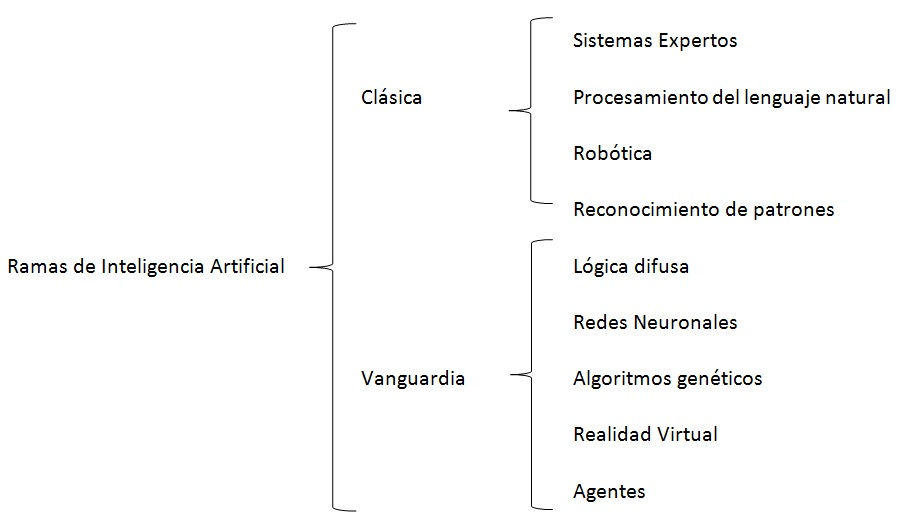
\includegraphics[width=8cm]{ramas_ia.png}}
	\caption{Ramas de la inteligencia artificial}
	\label{fig:ramas_ia}
\end{figure}

\textbf{Sistemas expertos.-}
son conocidos tambi�n como sistemas de conocimientos y estos programas inform�ticos aplican el proceso de razonamiento de un humano experto en la materia en la soluci�n de problemas espec�ficos. El modo de procesamiento de estos sistemas es en base a una gran base de datos y utilizando una heur�stica avanzada para la determinaci�n de las posibles soluciones a un problema.

\textbf{Procesamiento del lenguaje natural.-}
estos son sistemas capaces de reconocer, procesar y en cierto punto emular la comunicaci�n humana, estos sistemas buscan dejar el uso de lenguajes de programaci�n o conjunto de comandos, para procesar el lenguaje humano natural. Para procesar el lenguaje es necesario dividirlo, primero se obtiene la compresi�n del lenguaje natural, el cual investiga los m�todos para que una computadora sea capaz de entender las instrucciones de este lenguaje, la segunda etapa consiste en la generaci�n de lenguaje natural, aqu� es donde la maquina intenta comunicarse en el lenguaje humano.

\textbf{Rob�tica.-}
un robot es un dispositivo programado para realizar una tarea en espec�fico. Se dice que un robot est� adquiriendo inteligencia artificial si es capaz de responder a cambios en su entorno en lugar de seguir instrucciones programadas con anterioridad.

\textbf{Reconocimiento de patrones.-}
esta es la parte de la inteligencia artificial encargada del procesamiento visual de un entorno, las im�genes son captadas por c�maras y posteriormente procesadas para el reconocimiento de patrones del entorno.

\textbf{L�gica difusa.-}
es una forma matem�tica de representar el lenguaje natural, y el principio es generalizar la l�gica cl�sica haciendo que las variables tomen valores ling��sticos de verdad.

\textbf{Redes neuronales.-}
estas redes tratan de emular el comportamiento de las redes neuronales biol�gicas que poseen los humanos en su cerebro, partiendo de una neurona artificial y conect�ndola con otras para crear sinapsis entre ellas. 

\textbf{Algoritmos gen�ticos.-}
estos algoritmos son capaces de mutar para producir mejores respuestas a un entorno, estos sistemas tratan de imitar el proceso de selecci�n natural en el cual al ir mutando algunos genes se van obteniendo sistemas m�s capaces para un entorno. Su funci�n es seleccionar de una poblaci�n de soluciones candidatas e intentar producir nuevas generaciones de soluciones las cuales se buscan que sean mejores que las anteriores.

\textbf{Realidad virtual.-}
es la recreaci�n de un mundo artificial en tiempo real que puede ser captado por distintos canales sensoriales del espectador.
Agentes.- estos son peque�os programas que act�an como esp�as observando las acciones com�nmente realizadas por el usuario, estas acciones son almacenadas y registradas, si en dado caso se llega a dar una anomal�a el programa lanzara una alerta y dar� una serie de soluciones.

\subsection{Redes neuronales artificiales}

Las redes neuronales artificiales son un conjunto de neuronas creadas artificialmente para el desarrollo de inteligencia artificial en una computadora.
 
Estas redes est�n basadas en las redes biol�gicas del cerebro humano, modelando todos los factores biol�gicos de las neuronas.

\begin{figure}[htbp]
	\centerline{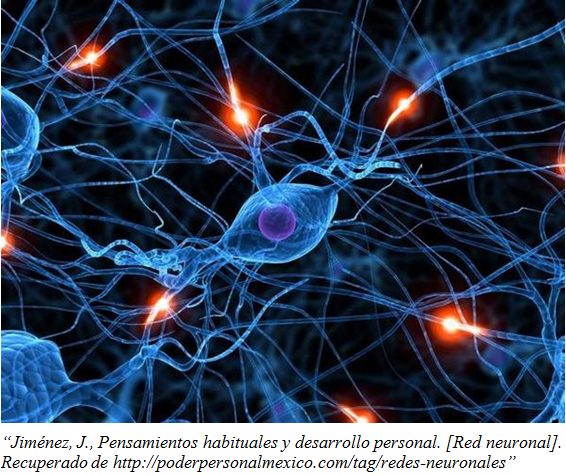
\includegraphics[width=7cm]{red_bio.png}}
	\caption{Red neuronal biol�gica}
	\label{fig:red_bio}
\end{figure}

Debido a su dise�o las redes son capaces de aprender de la experiencia, de generalizar de casos anteriores a nuevos casos, de abstraer caracter�sticas esenciales a partir de entradas que representan en ocasiones informaci�n irreverente.

La capacidad de aprendizaje adaptativo es una caracter�stica fundamental de las redes neuronales y les permiten llevar a cabo ciertas tareas mediante un entrenamiento previo, pueden aprender a diferenciar patrones y generalizar a partir de estos. Son considerados sistemas din�micos ya que son capaces de adaptarse a nuevas condiciones de entrada.

Tienen una alta tolerancia a fallos ya que son capaces de detectar patrones aun cuando estos patrones posean ruido, distorsi�n o simplemente est�n incompletos. Estos programas son capaces de seguir funcionando incluso si parte de la red presente fallas.

La informaci�n se almacena de forma distribuida en las conexiones de las neuronas, provocando redundancia de informaci�n, es decir se guardara sus valores en base a la funci�n de activaci�n que posee cada neurona, de esta manera si una neurona es destruida o presenta fallas, las otras neuronas podr�n aprender la informaci�n de la neurona que fallo.

Las neuronas humanas poseen diferentes secciones:

\begin{figure}[htbp]
	\centerline{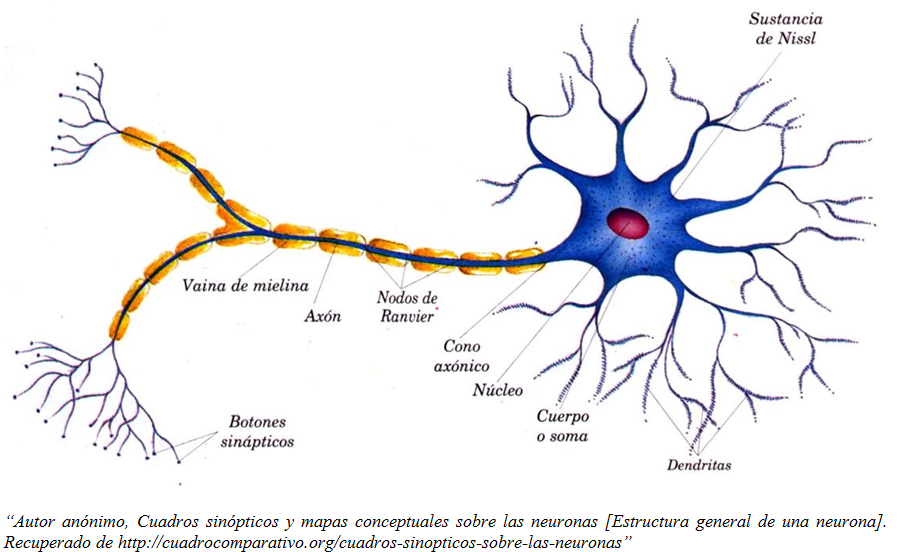
\includegraphics[width=8cm]{estruc_neu.png}}
	\caption{Estructura general de una neurona}
	\label{fig:estruc_neu}
\end{figure}

En una neurona artificial se busca la emulaci�n de las principales secciones de una neurona las cuales son:

\begin{itemize}
	\item \textbf{Cuerpo.-} Se encarga de producir un impulso el�ctrico en base a las entradas de la neurona.
	\item \textbf{Dendritas.-} son filamentos capaces de crear conexiones con otras neuronas.
	\item \textbf{Ax�n.-} Es el encargado de transmitir el impulso el�ctrico generado por el cuerpo.
\end{itemize}

A continuaci�n se muestra una imagen de como lucir�a una neurona artificial:

\begin{figure}[htbp]
	\centerline{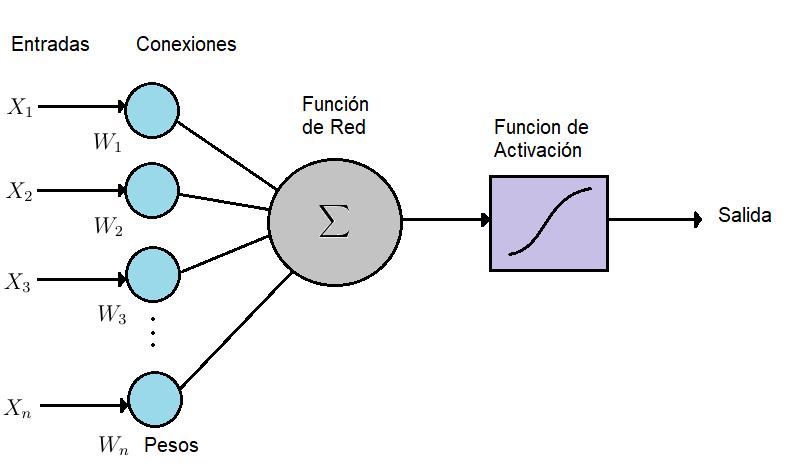
\includegraphics[width=8cm]{neu_art.png}}
	\caption{Neurona Artificial}
	\label{fig:neu_art}
\end{figure}

Esta neurona posee las siguientes secciones:

\begin{itemize}
	\item \textbf{X1, X2, \ldots,Xn .-} Son las entradas de la neurona.
	\item \textbf{W1, W2, \ldots, Wn.-} Pesos espec�ficos que tendr� cada entrada, esto hace que las entradas no valgan lo mismo ponderadamente.
	\item \textbf{Funci�n de red.-} Esta es una funci�n de sumatoria de las entradas.
	\item \textbf{Funci�n de activaci�n.-} Si la suma de las entradas es mayor o igual que el umbral definido por esta funci�n se tendr� una se�al a la salida.
\end{itemize}

La salida de la neurona viene dada por esta ecuaci�n:

\begin{equation}
y_j = f(\sum_{i=1}^{n}(W_{ij}x_i + \theta_j))
\label{ec:neu_out}
\end{equation}

Una red neuronal no es m�s que la interconexi�n de varias neuronas artificiales, en la cual podemos identificar al menos tres secciones:

\begin{itemize}
	\item \textbf{Capa de entrada.-} En esta capa se procesan todas las entradas, y si estas entradas son capaces de excitar las neuronas de esta capa se producir� una se�al de salida.
	\item \textbf{Capa oculta.-} En esta capa se encuentran las neuronas encargadas del aprendizaje de la red.
	\item \textbf{Capa de salida.-} Esta neurona o neuronas de salida tendr�n la salida del sistema.
\end{itemize}

La forma en que las redes aprenden es mediante la modificaci�n de los pesos de las entradas.

Las redes neuronales artificiales han ido evolucionando con el paso del tiempo, hoy en d�a existen muchos modelos de redes neuronales, todas ellas con ventajas y desventajas si son comparadas entre ellas.

\subsubsection{Aprendizaje de las redes neuronales}

%TODO: Rf
El procedimiento utilizado para llevar a cabo el proceso de aprendizaje en una red neuronal se denomina entrenamiento.

El problema de aprendizaje en las redes neuronales se formula en t�rminos de la minimizaci�n de la funci�n de error (o p�rdida) asociada.

Normalmente, esta funci�n est� compuesta por dos t�rminos, uno que eval�a c�mo se ajusta la salida de la red neuronal al conjunto de datos de que disponemos, y que se denomina t�rmino de error, y otro que se denomina t�rmino de regularizaci�n, y que se utiliza para evitar el sobreaprendizaje por medio del control de la complejidad efectiva de la red neuronal.

Por supuesto, el valor de la funci�n de error depende por completo de los par�metros de la red neuronal: los pesos sin�pticos entre neuronas, y los bias asociados a ellas, que, como suele ser ya habitual, se pueden agrupar adecuadamente en un �nico vector de peso de la dimensi�n adecuada, que denotaremos por $w$. En este sentido, podemos escribir $f(w)$ para indicar que el valor del error que comete la red neuronal depende de los pesos asociados a la misma. Con esta formalizaci�n, nuestro objetivo es encontrar el valor $w^{*}$ para el que se obtiene un m�nimo global de la funci�n $f$, convirtiendo el problema de aprendizaje en un problema de optimizaci�n.

En general, la funci�n de error es una funci�n no lineal, por lo que no disponemos de algoritmos sencillos y exactos para encontrar sus m�nimos. En consecuencia, tendremos que hacer uso de una b�squeda a trav�s del espacio de par�metros que, idealmente, se aproxime de forma iterada a a un (error) m�nimo de la red para los par�metros adecuados.

De esta forma, se comienza con una red neuronal con alg�n vector inicial de par�metros (a menudo elegido al azar), a continuaci�n se genera un nuevo vector de par�metros, esperando que con ellos la funci�n de error se reduzca (aunque dependiendo del m�todo elegido, no es obligatorio, y temporalmente se puede admitir un empeoramiento del error siempre y cuando conduzca a una disminuci�n posterior m�s acusada). Este proceso se repite, normalmente, hasta haber reducido el error bajo un umbral tolerable, o cuando se satisfaga una condici�n espec�fica de parada.

El Descenso del Gradiente es el algoritmo de entrenamiento m�s simple y tambi�n el m�s extendido y conocido. Solo hace uso del vector gradiente, y por ello se dice que es un m�todo de primer orden.

Este m�todo para construir el punto $w_{i+1}$ a partir de wi se traslada este punto en la direcci�n de entrenamiento $d_i=-g_i$. Es decir:

\begin{equation}
w_{i+1} = w_{i} - g_{i}v_{i}
\label{ec:grad}
\end{equation}

Donde el par�metro $v$ se denomina tasa de entrenamiento, que puede fijarse a priori o calcularse mediante un proceso de optimizaci�n unidimensional a lo largo de la direcci�n de entrenamiento para cada uno de los pasos (aunque esta �ltima opci�n es preferible, a menudo se usa un valor fijo, $v_{i}=v$ con el fin de simplificar el proceso).

Aunque es muy sencillo, este algoritmo tiene el gran inconveniente de que, para funciones de error con estructuras con valles largos y estrechos, requiere muchas iteraciones. Se debe a que, aunque la direcci�n elegida es en la que la funci�n de error disminuye m�s r�pidamente, esto no significa que necesariamente produzca la convergencia m�s r�pida.

Por ello, es el algoritmo recomendado cuando tenemos redes neuronales muy grandes, con muchos miles de par�metros, ya que s�lo almacena el vector gradiente (de tama�o n).
%http://www.cs.us.es/~fsancho/?e=165
%Rf

\subsection{Deep Learning}

Deep Learning usa redes neuronales con muchas capas para lograr aprendizajes m�s complejos. Este comportamiento asemeja la forma en que el cerebro humano toma decisiones, el cual usa la interconexi�n de varias capas de neuronas para realizar actividades complejas.
Dentro de las redes de Deep Learning se tienen 2 tipos muy usados en la actualidad:

\begin{itemize}
	\item \textbf{Redes convolucionales (CNN).-} Este tipo de redes usa la convoluci�n en varias de sus capaz para lograr el procesamiento de par�metros que se pueden representar en un espacio $R^2$, un ejemplo claro de esto son las im�genes y v�deos, por lo tanto si se quiere hacer una clasificaci�n o reconocimiento de im�genes, este tipo de redes nos proporcionan una buena herramienta de procesamiento.
	\item \textbf{Redes recurrentes (RNN).-} Este tipo de redes son muy usadas cuando se busca analizar una secuencia de datos, estas redes poseen memoria y una retroalimentaci�n de la salida a la entrada.  
\end{itemize}

\subsection{Redes neuronales recurrentes}

%TODO: Rf
La idea detr�s de las RNN es hacer uso de la informaci�n secuencial. En una red neuronal tradicional suponemos que todas las entradas (y salidas) son independientes entre s�. Pero para muchas tareas eso es una muy mala idea. Si quieres predecir la siguiente palabra en una oraci�n, es mejor que conozcas qu� palabras vienen antes. Las RNN se llaman recurrentes porque realizan la misma tarea para cada elemento de una secuencia, y la salida depende de los c�lculos previos. Otra forma de pensar acerca de las RNN es que tienen una "memoria" que captura informaci�n sobre lo que se ha calculado hasta ahora. En teor�a, los RNN pueden hacer uso de la informaci�n en secuencias arbitrariamente largas, pero en la pr�ctica se limitan a mirar hacia atr�s solo unos pocos pasos.

La decisi�n de una red recurrente alcanzada en el paso de tiempo t-1 afecta la decisi�n que alcanzar� un momento m�s tarde en el paso de tiempo t. Entonces, las redes recurrentes tienen dos fuentes de entrada, el presente y el pasado reciente, que se combinan para determinar c�mo responden a los datos nuevos, de forma similar a como lo hacemos en la vida.

Esa informaci�n secuencial se conserva en el estado oculto de la red recurrente, que logra abarcar muchos pasos de tiempo a medida que avanza para afectar el procesamiento de cada nuevo ejemplo. Est� encontrando correlaciones entre eventos separados por muchos momentos, y estas correlaciones se llaman "dependencias a largo plazo", porque un evento en el tiempo depende de, y es una funci�n de, uno o m�s eventos que vinieron antes. Una forma de pensar acerca de las RNN es esta: son una forma de compartir pesos a lo largo del tiempo.

As� como la memoria humana circula invisiblemente dentro de un cuerpo, afectando nuestro comportamiento sin revelar su forma completa, la informaci�n circula en los estados ocultos de las redes recurrentes.

Describiremos el proceso de llevar la memoria hacia adelante matem�ticamente:

\begin{equation}
h_t = \phi(Wx_t + Uh_{t-1})
\label{ec:mem_neu}
\end{equation}

El estado oculto en el paso de tiempo $t$ es $h_t$. Es una funci�n de la entrada al mismo tiempo paso $x_t$, modificada por una matriz de ponderaci�n W (como la que usamos para las redes feedforward) agregada al estado oculto del paso de tiempo anterior $h_{t-1}$ multiplicado por su propio estado oculto matriz U de estado oculto, tambi�n conocida como matriz de transici�n y similar a una cadena de Markov. Las matrices de peso son filtros que determinan la importancia de acuerdo tanto con la entrada actual como con el estado oculto pasado. El error que generan volver� a trav�s de la propagaci�n inversa y se usar� para ajustar sus ponderaciones hasta que el error no pueda bajar m�s.

Debido a que este ciclo de retroalimentaci�n ocurre en cada paso de la serie, cada estado oculto contiene rastros no solo del estado oculto anterior, sino tambi�n de todos los que precedieron a $h_{t-1}$ mientras la memoria pueda persistir.

\subsubsection{LSTM}

A mediados de los a�os 90, los investigadores alemanes Sepp Hochreiter y Juergen Schmidhuber propusieron una variaci�n de la red recurrente con las denominadas unidades de memoria a largo plazo, o LSTM, como una soluci�n al problema del gradiente de fuga.

Los LSTM ayudan a preservar el error que se puede volver a propagar a trav�s del tiempo y las capas. Al mantener un error m�s constante, permiten que las redes recurrentes contin�en aprendiendo durante muchos pasos de tiempo (m�s de 1000), abriendo as� un canal para vincular causas y efectos de forma remota. Este es uno de los desaf�os centrales para el aprendizaje autom�tico y la IA, ya que los algoritmos se enfrentan con frecuencia a entornos en los que las se�ales de recompensa son dispersas y diferidas, como la vida misma.

Los LSTM contienen informaci�n fuera del flujo normal de la red recurrente en una celda cerrada. La informaci�n puede almacenarse, escribirse o leerse desde una celda, al igual que los datos en la memoria de una computadora. La c�lula toma decisiones sobre qu� almacenar y cu�ndo permitir las lecturas, escrituras y borraduras, a trav�s de puertas que se abren y cierran. Sin embargo, a diferencia del almacenamiento digital en computadoras, estas puertas son an�logas, implementadas con la multiplicaci�n de elementos por sigmoides, que est�n todas en el rango de 0-1. Siendo Analogica tiene la ventaja sobre digital de ser diferenciable y, por lo tanto, adecuado para la propagaci�n inversa.

Esas puertas act�an sobre las se�ales que reciben, y de forma similar a los nodos de la red neuronal, bloquean o transmiten informaci�n en funci�n de su fuerza e importaci�n, que filtran con sus propios conjuntos de ponderaciones. Esos pesos, como los pesos que modulan los estados de entrada y ocultos, se ajustan a trav�s del proceso de aprendizaje de redes recurrentes. Es decir, las c�lulas aprenden cu�ndo permiten que los datos entren, salgan o se eliminen a trav�s del proceso iterativo de hacer conjeturas, volver a propagar el error y ajustar los pesos mediante el descenso del gradiente.
% https://skymind.ai/wiki/lstm
%Rf

\subsection{Composici�n musical}

La composici�n musical esta catalogado como un arte que tiene como objeto crear nuevas piezas musicales.

Un m�sico puede optar por varios caminos para la creaci�n de su obra, existen m�sicos que se basan en su simple sentido com�n y crean canciones liricamente, sin embargo el proceso formal de composici�n involucra todos los conceptos musicales b�sicos de la teor�a musical.

\subsection{Teor�a musical}

La teor�a musical es el estudio de los elementos que conforman la m�sica. En esta teor�a se analizan todos los sonidos involucrados para la creaci�n, an�lisis y composici�n musical.

La m�sica es un arte que se basa en 2 elementos: 

\begin{itemize}
	\item Los sonidos
	\item Los silencios
\end{itemize}

Los sonidos tienen diferentes propiedades las cuales se describen a continuaci�n:

\begin{itemize}
	\item \textbf{Altura.-} un sonido puede ser agudo, medio o grave, dependiendo de la altura de su nota.
	\item \textbf{Duraci�n.-} un sonido debe de tener una duraci�n la cual se expresa en unidades de tiempo.
	\item \textbf{Intensidad.-} esto se refiere al volumen del sonido, puede ser d�bil o fuerte.
	\item \textbf{Timbre.-} se le conoce como timbre o color del sonido a como un sonido con la misma nota suena diferente dependiendo del instrumento usado para su interpretaci�n.  
\end{itemize}

Los silencios a su vez su �nica propiedad intr�nseca es la duraci�n, es decir en un silencio lo �nico que se mide es la duraci�n del mismo.

\subsection{Notas musicales}

Las notas es un sistema que se usa para la representaci�n de los diferentes sonidos en la m�sica. En el mundo occidental se usa un sistema de 12 notas, los cuales pueden ser repetidos con diferentes alturas para generar una gama muy amplia de sonidos.
Dentro de este sistema de 12 notas tenemos las notas naturales y las notas con alteraciones.
Las notas naturales son:

Do, Re, Mi, Fa, Sol, La, Si   (7 notas)

Las alteraciones no son m�s que agregar o quitar medios tonos a una nota, para eso se usan los siguientes s�mbolos:

\begin{itemize}
	\item \textbf{\# (sostenido).-} se agrega $1/2$ tono a una nota.
	\item \textbf{x (doble sostenido).-} Se agrega 1 tono a una nota.
	\item \textbf{$\flat$ (bemol).-} se disminuye $1/2$ tono a una nota.
	\item \textbf{$\flat\flat$ (doble bemol).-} Se disminuye 1 tono a una nota.  
\end{itemize}

Usando los s�mbolos anteriores podemos definir las siguientes notas con alteraciones:

Do\#, Re\#, Fa\#, Sol\#, La\#  (5 notas)

Como se puede observar tanto Mi y Si no tienen sonidos con alteraciones ascendentes, ya que los sonidos producidos por estas alteraciones son igual al de las notas consecutivas, a este tipo de sonidos iguales se les conoce como notas enarm�nicas.

Por ejemplo:

\begin{itemize}
	\item Mi\# sonar�a exactamente igual que un Fa.
	\item Si\# sonar�a exactamente igual que un Do.  
\end{itemize}

Tambi�n las notas con alteraciones pueden ser representadas usando el s�mbolo de bemol (b), es decir restando medio tono a una nota. En este caso se tendr�an las notas con alteraciones de la siguiente manera:

Re$_\flat$, Mi$_\flat$, Sol$_\flat$, La$_\flat$, Si$_\flat$      (5 notas)

Como se mencion� anteriormente las notas que en sonido son exactamente iguales pero en nomenclatura son diferentes se conocen como notas enarm�nicas, de tal manera que las 5 notas con alteraciones que se describieron se pueden hacer una comparaci�n del sonido de las mismas, siendo as� se tiene:

\begin{itemize}
	\item Do\#  suena exactamente igual que Re$_\flat$.
	\item Re\# suena exactamente igual que Mi$_\flat$. 
	\item Fa\# suena exactamente igual que Sol$_\flat$. 
	\item Sol\# suena exactamente igual que La$_\flat$. 
	\item La\# suena exactamente igual que Si$_\flat$.   
\end{itemize}

Podemos ver la relaci�n de tonos y semitonos (1/2 tonos) en la siguiente figura:

\begin{figure}[htbp]
	\centerline{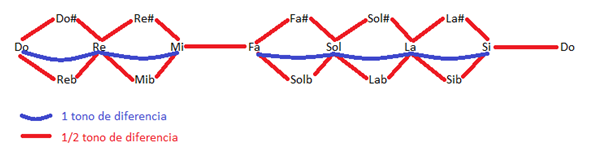
\includegraphics[width=8cm]{tonos.png}}
	\caption{Relacion de tonos y semitonos}
	\label{fig:tonos}
\end{figure}

Como se puede observar entre Mi y Fa existe un semitono, al igual que entre Si y Do.

El pentagrama es un sistema de cinco l�neas y cuatro espacios para escribir m�sica:

\begin{figure}[htbp]
	\centerline{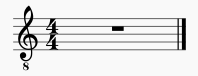
\includegraphics[width=8cm]{pentagrama.png}}
	\caption{Pentagrama}
	\label{fig:pentagrama}
\end{figure}

Este sistema puede tener diferentes elementos dentro de los principales tenemos:

\begin{itemize}
	\item Clave.
	\item Comp�s.
	\item Armadura. 
	\item Notas.
\end{itemize}

\subsection{Claves musicales}

Las claves musicales se usan para darle nombre y altura a las notas musicales dentro de un pentagrama.

Las claves m�s usadas en la m�sica son: la clave de Sol, la clave de Fa y la clave de Do.

La clave de Sol se usa en instrumentos agudos como la guitarra, viol�n, entre otros. Esta clave normalmente se escribe empezando en la segunda l�nea del pentagrama para formar una especie de G. El hecho de que esta clave se escriba en la segunda l�nea establece que esa l�nea ser� llamada como el nombre de la clave, en este caso Sol:

\begin{figure}[htbp]
	\centerline{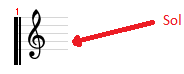
\includegraphics[width=4cm]{clave_sol.png}}
	\caption{Clave de Sol en 2da. Linea}
	\label{fig:clave_sol}
\end{figure}

La clave de Fa es usada en instrumentos m�s graves, tales como el contrabajo, el bajo, etc. Normalmente se escribe empezando en la cuarta l�nea, de tal manera que esta l�nea tomara el nombre de Fa:

\begin{figure}[htbp]
	\centerline{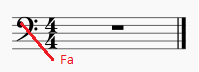
\includegraphics[width=4cm]{clave_fa.png}}
	\caption{Clave de Fa en 4ta. Linea}
	\label{fig:clave_fa}
\end{figure}

La clave de Do es usada com�nmente para las voces, y esta clave se escribe en diferentes l�neas dependiendo del timbre de la voz, para un tenor se usa la clave de Do en 4ta l�nea, mientras que para un soprano normalmente la clave se usa en 3ra o 2da l�nea:

\begin{figure}[htbp]
	\centerline{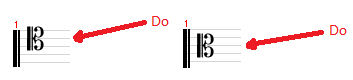
\includegraphics[width=8cm]{clave_do.png}}
	\caption{Clave de Do en 4ta. y 3ra. linea}
	\label{fig:clave_do}
\end{figure}

A partir de estas claves se le puede poner nombre a las diferentes l�neas y espacios del pentagrama, por ejemplo en la clave de sol en segunda l�nea, el pentagrama quedar�a de la siguiente forma:

\begin{figure}[htbp]
	\centerline{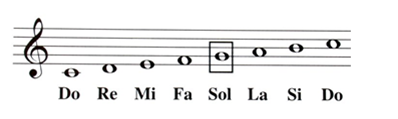
\includegraphics[width=8cm]{notas_clave_sol.png}}
	\caption{Nombre de las notas en un pentagrama con clave de Sol}
	\label{fig:notas_clave_sol}
\end{figure}

\subsection{Compases y tiempo}

El comp�s se puede definir como la unidad m�trica de la m�sica, es la que nos dice que tiempo llevara la canci�n.

Existen una infinidad de compases los cuales podemos clasificar en dos grandes grupos:

\begin{itemize}
	\item Compases regulares.
	\item Compases irregulares.
\end{itemize}

Los compases regulares est�n regidos por formas regulares las cuales dictan el tiempo, mientras que en los compases irregulares hay que determinar la base de tiempo de forma indirecta.

Cada nota puede tener un valor de tiempo y este valor estar� determinado por el comp�s que se est� utilizando, por ejemplo en un comp�s de 4/4 las figuras musicales tendr�n los siguientes valores:

\begin{figure}[htbp]
	\centerline{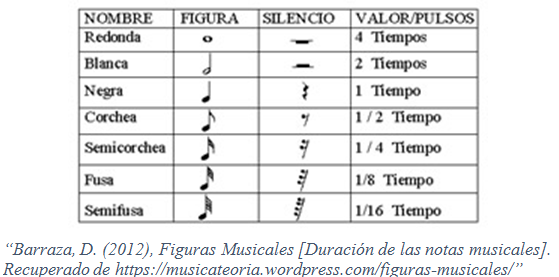
\includegraphics[width=8cm]{dura_notas.png}}
	\caption{Duraci�n de las notas musicales}
	\label{fig:dura_notas}
\end{figure}

Como se puede observar para cada figura musical existe su silencio correspondiente, el cual tendr� el mismo valor solo que este caso no se producir� sonido alguno.

Podemos tener tambi�n los valores relativos de estas notas respecto a otras notas:

\begin{figure}[htbp]
	\centerline{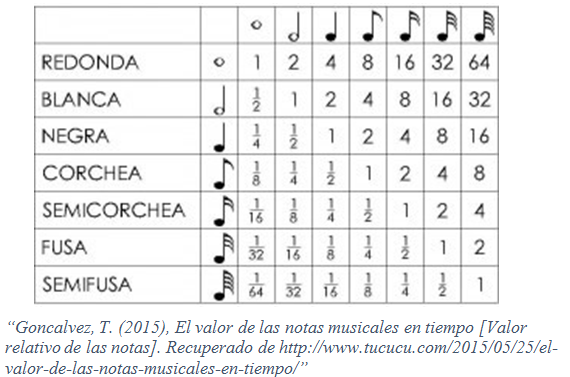
\includegraphics[width=8cm]{valor_rel.png}}
	\caption{Valor relativo de las notas}
	\label{fig:valor_rel}
\end{figure}

De tal manera que en un comp�s tendremos dos datos los cuales se describen a continuaci�n:

\begin{figure}[htbp]
	\centerline{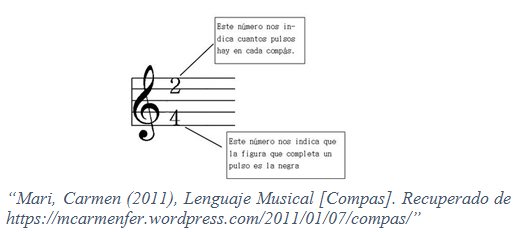
\includegraphics[width=8cm]{compas.png}}
	\caption{Compas}
	\label{fig:valor_rel}
\end{figure}

Se puede ver que este compas tendr� 2 pulsos y el valor de cada pulso ser� de un tiempo de negra, ya que el valor relativo de la negra respecto a la redonda es de $1/4$.

Otro punto a considerar en los compases es que estos tienen tiempos fuertes, semifuertes y d�biles. La cuadratura de una armon�a usa estos tiempos para indicar los cambios que se deben de hacer.

Este es un ejemplo de los tiempos en compases de $4/4$, $3/4$ y $2/4$: 

\begin{figure}[htbp]
	\centerline{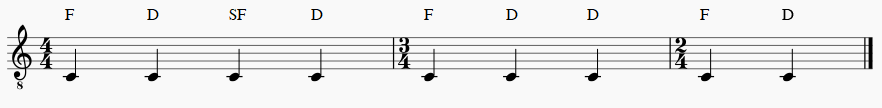
\includegraphics[width=8cm]{tiempos_fd.png}}
	\caption{Tiempos fuertes y d�biles}
	\label{fig:tiempos_fd}
\end{figure}

\subsection{Escalas}

Las escalas son una serie de notas musicales que siguen un orden establecido por intervalos desde una nota base. En el mundo de la m�sica hay una infinidad de escalas pero todas parten de la escala mayor de Do:

\begin{figure}[htbp]
	\centerline{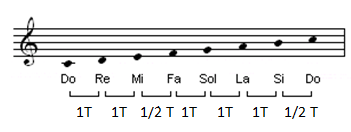
\includegraphics[width=8cm]{escala.png}}
	\caption{Escala de Do Mayor}
	\label{fig:escala}
\end{figure}

En la escala mayor se tiene los siguientes intervalos: tono, tono, semitono, tono, tono, tono, semitono, si esta f�rmula la aplicamos con las otras notas musicales podremos construir todas las escalas mayores.

Por ejemplo la escala de sol mayor quedar�a de la siguiente manera:

\begin{figure}[htbp]
	\centerline{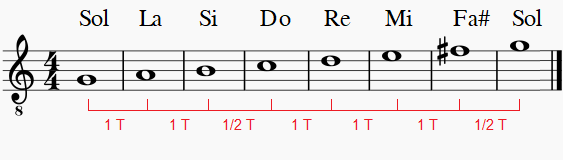
\includegraphics[width=8cm]{escala_sol.png}}
	\caption{Escala de Sol Mayor}
	\label{fig:escala_sol}
\end{figure}

Para poder completar el tono completo de la f�rmula de la escala mayor entre Mi y Fa se tuvo que poner una alteraci�n en la nota de Fa.

La �nica escala mayor que no posee alteraciones es la escala mayor de Do, de ah� en m�s todas las dem�s escalas mayores tendr�n al menos una alteraci�n.

Las escalas menores parten de la escala mayor obteniendo su sexta nota y siguiendo las mismas notas de la escala mayor. Estas escalas menores se les conocen como menores relativas, ya que se basan en una escala mayor para su formaci�n.

Por ejemplo la escala relativa de Do mayor seria La menor y esta escala posee exactamente las mismas notas que la escala mayor solamente que empieza desde la nota de La:

En este caso las notas son: La, Si, Do, Re, Mi, Fa, Sol, La.

\begin{figure}[htbp]
	\centerline{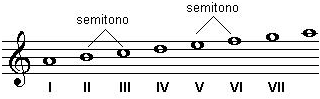
\includegraphics[width=8cm]{escala_la_men.png}}
	\caption{Escala de La menor}
	\label{fig:escala_la_men}
\end{figure}

Esta relatividad puede ser usada con todas las escalas mayores para obtener sus relativas menores.

A pesar que las escalas mayores y menores poseen las mismas notas no deben ser nunca confundidas ya que el sonido final producido es muy diferente, mientras las escalas mayores se usan para canciones se puede decir hasta cierto punto alegres, las escalas menores normalmente acompa�an melod�as melanc�licas, esto no es en todos los casos.

\subsection{Armaduras}

Todas las alteraciones de una escala se pueden juntar al inicio del pentagrama para dar lugar a lo que se conoce como armaduras.

Estas armaduras indicaran que todas las notas que poseen alteraciones las mantendr�n a lo largo de toda la canci�n.

Debido a que las escalas mayores y sus relativas menores poseen las mismas alteraciones por lo tanto comparten tambi�n la misma armadura:

\begin{figure}[htbp]
	\centerline{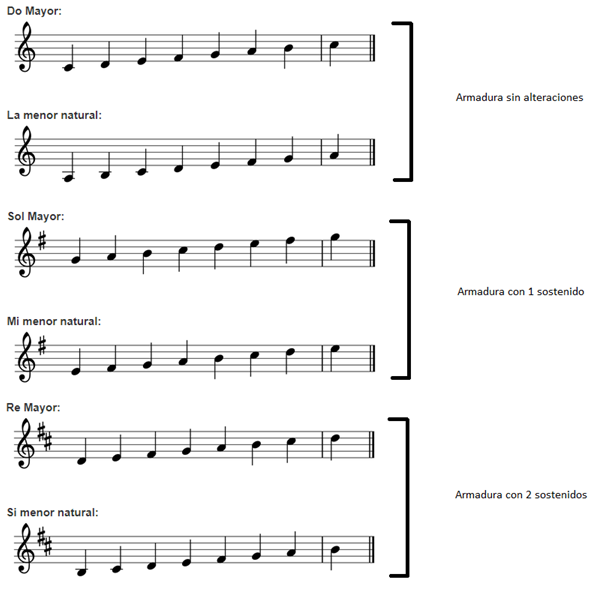
\includegraphics[width=6cm]{armadura_sost.png}}
	\caption{Armaduras relativas con sostenidos}
	\label{fig:armadura_sost}
\end{figure}

Tambi�n podemos tener armaduras con bemoles:

\begin{figure}[htbp]
	\centerline{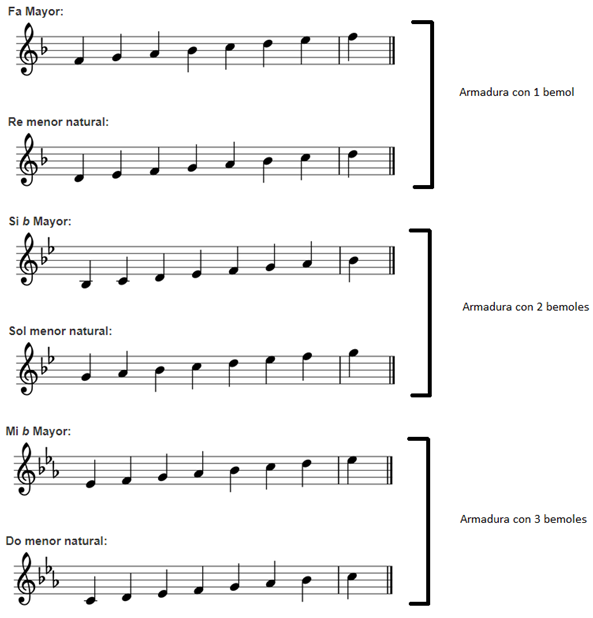
\includegraphics[width=6cm]{armadura_bem.png}}
	\caption{Armaduras relativas con bemoles}
	\label{fig:armadura_bem}
\end{figure}

\subsection{Tonalidades}

La tonalidad de una canci�n se basa en la escala base de la canci�n y esta la podemos averiguar viendo la armadura que posee la canci�n, aunque como se vio anteriormente las escalas mayores y sus relativas poseen la misma armadura, as� que antes de definir la tonalidad en base a la armadura tambi�n se debe de hacer un an�lisis de la interacci�n de las notas en la canci�n.

Dentro de las tonalidades tenemos tonalidades mayores y menores, por ejemplo si vemos un pentagrama el cual no posee alteraciones podr�amos asumir que la canci�n esta en Do mayor o en La menor, el siguiente paso ser�a ver la interacci�n de las notas en la canci�n para determinar correctamente la tonalidad.

\subsection{Melod�as y Armon�as}

Una melod�a es una sucesi�n de notas de forma ascendente o descendente que llevan cierta cordura. 

Las melod�as suelen estar formadas por frases y generalmente se repiten a lo largo de una canci�n variando algunas notas intermedias. En este caso se trata de una sucesi�n de notas que no son tocadas al mismo tiempo sino que una nota es tocada despu�s de la otra.

Las armon�as son una conjunci�n de sonidos tocados al mismo tiempo, normalmente la sucesi�n de varios acordes arm�nicos est� ligado directamente con la melod�a de la canci�n.

La armon�a ha cambiado considerablemente desde la �poca de la m�sica barroca hasta la m�sica moderna, anteriormente para generar sistemas arm�nicos se usaban varios instrumentos tocando una nota en espec�fico y la conjunci�n de todos los sonidos daba como resultado la armon�a, actualmente la armon�a es creada a partir de acordes de instrumentos que puedan generar este tipo de condiciones.

Esta es una comparativa para diferenciar entre lo que ser�a una melod�a y una armon�a:

\begin{figure}[htbp]
	\centerline{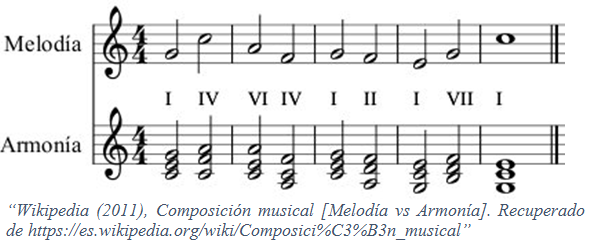
\includegraphics[width=8cm]{melo_armo.png}}
	\caption{Melod�a y Armon�a}
	\label{fig:melo_armo}
\end{figure}

\subsection{Formato MIDI}

%TODO: Rf
% Deep Learning Techniques for Music Generation - {A} Survey  <- Bibliografia

MIDI (Interfaz digital de instrumentos musicales) es un est�ndar t�cnico que describe un protocolo, una interfaz digital y conectores para la interoperabilidad entre varios instrumentos musicales electr�nicos, software y dispositivos. MIDI transmite mensajes de eventos que especifican informaci�n de notas (como tono y velocidad), as� como se�ales de control para par�metros (como volumen, vibrato y se�ales de reloj). Hay cinco tipos de mensajes y aqu� solo consideramos el tipo de Canal de voz, que transmite datos de rendimiento en tiempo real a trav�s de un solo canal. Dos mensajes importantes son:

\begin{itemize}
	\item \textbf{Note on.-} Indica que una nota debe ser reproducida. Contiene la informaci�n de estado (n�mero de canal, especificado por un entero dentro de [0 15] y dos valores de datos: un n�mero de nota MIDI (el tono de la nota, un entero dentro de [0 127]) y una velocidad (que indica c�mo la nota es reproducida, un entero dentro de [0 127]). Un ejemplo es <Note on, 0, 60, 50> que interpreta como: "en el canal 1, comienza a reproducir un C medio con una velocidad de 50".
	\item \textbf{Note off.-} Indica que una nota termina. En esa situaci�n, la velocidad indica qu� tan r�pido se libera la nota. Un ejemplo es <Note off, 0, 60, 20> que interpreta como: "en el canal 1, deja de reproducir un C medio con una velocidad de 20". 
\end{itemize}

Cada evento de nota est� realmente incrustado en un fragmento de pista, una estructura de datos que contiene un valor de tiempo delta que especifica la informaci�n de temporizaci�n y el evento en s�. Un valor de tiempo delta representa la posici�n de tiempo, como un valor absoluto, del evento y podr�a representar:

\begin{itemize}
	\item \textbf{Metrical time.-} Representa el numero de pulsos desde el comienzo. Una referencia llamada divisi�n y es definida en el encabezado del archivo, especificando cuantos pulsos por nota de cuarto.
	\item \textbf{time-code-based time.-} Representa el tiempo relacionado con horas, minutos y segundos de la canci�n. 
\end{itemize}

Un ejemplo de un extracto de un archivo MIDI y su partitura correspondiente es mostrado en las siguientes figuras. La divisi�n ah sido puesta en 384 pulsos por cuarto de nota lo cual corresponde a 96 pulsos por un octavo de nota:

\begin{figure}[htbp]
	\centerline{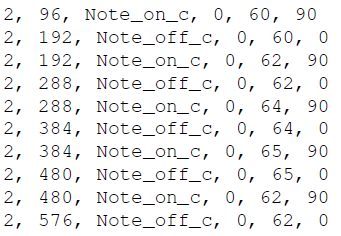
\includegraphics[width=6cm]{extract_midi.png}}
	\caption{Extracto de un formato MIDI}
	\label{fig:extract_midi}
\end{figure}

\begin{figure}[htbp]
	\centerline{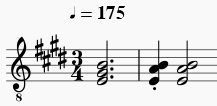
\includegraphics[width=6cm]{repres_midi.png}}
	\caption{Partitura correspondiente al extracto MIDI}
	\label{fig:repres_midi}
\end{figure}

%Rf

Dentro del formato MIDI se pueden representar en cada track un instrumento diferente eh independiente de los dem�s, esto permite una f�cil manipulaci�n de los diferentes instrumentos. A continuaci�n se muestra una tabla de todos los instrumentos que pueden ser representados en este formato:

\begin{figure}[htbp]
	\centerline{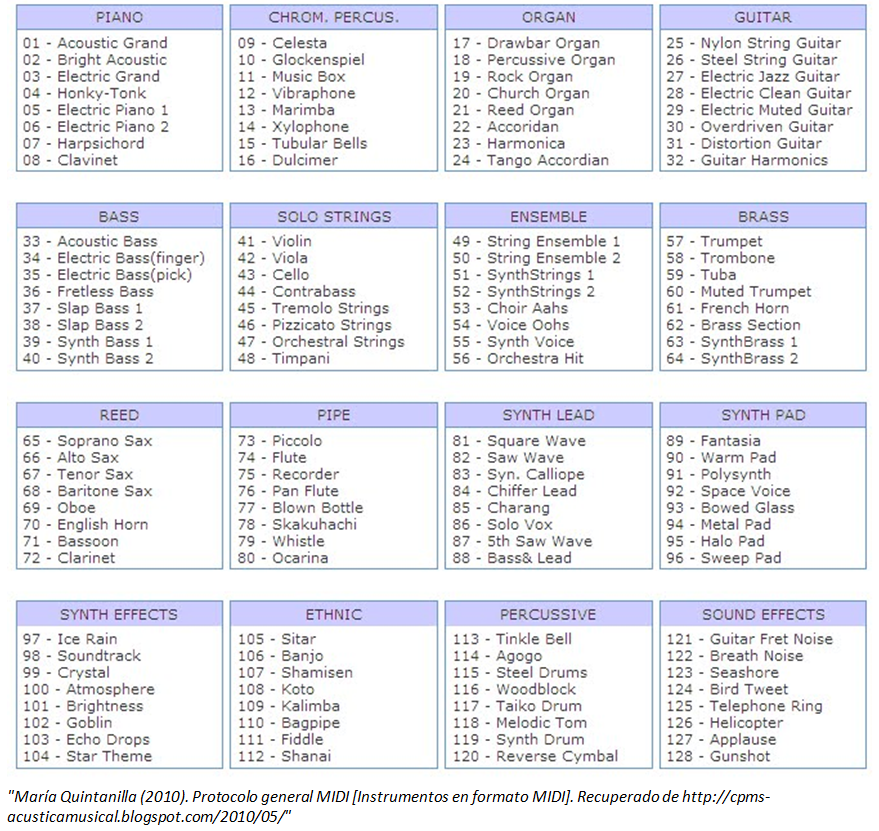
\includegraphics[width=12cm]{instr_midi.png}}
	\caption{Instrumentos en formato MIDI}
	\label{fig:instr_midi}
\end{figure}
%IMD PNA http://na.support.keysight.com/pna/help/latest/Applications/Swept_IMD_Configure_External_Source_and_Combiner.htm
\chapter{Teor�a musical}



%%-----------------------------------------------------------------------


%\section{}

La teor�a musical es el estudio de los elementos que conforman la m�sica. En esta teor�a se analizan todos los sonidos involucrados para la creaci�n, an�lisis y composici�n musical.

La m�sica es un arte que se basa en 2 elementos: 

\begin{itemize} [noitemsep]
	\item Los sonidos
	\item Los silencios
\end{itemize}

Los sonidos tienen diferentes propiedades las cuales se describen a continuaci�n:

\begin{itemize}
	\item \textbf{Altura.-} un sonido puede ser agudo, medio o grave, dependiendo de la altura de su nota.
	\item \textbf{Duraci�n.-} un sonido debe de tener una duraci�n la cual se expresa en unidades de tiempo.
	\item \textbf{Intensidad.-} esto se refiere al volumen del sonido, puede ser d�bil o fuerte.
	\item \textbf{Timbre.-} se le conoce como timbre o color del sonido a como un sonido con la misma nota suena diferente dependiendo del instrumento usado para su interpretaci�n.  
\end{itemize}

Los silencios a su vez su �nica propiedad intr�nseca es la duraci�n, es decir en un silencio lo �nico que se mide es la duraci�n del mismo.

\section{Composici�n musical}

La composici�n musical esta catalogado como un arte que tiene como objeto crear nuevas piezas musicales.

Un m�sico puede optar por varios caminos para la creaci�n de su obra, existen m�sicos que se basan en su simple sentido com�n y crean canciones liricamente, sin embargo el proceso formal de composici�n involucra todos los conceptos musicales b�sicos de la teor�a musical, los cuales se describir�n a continuaci�n.

\subsection{Notas musicales}

Las notas es un sistema que se usa para la representaci�n de los diferentes sonidos en la m�sica. En el mundo occidental se usa un sistema de 12 notas, los cuales pueden ser repetidos con diferentes alturas para generar una gama muy amplia de sonidos.
Dentro de este sistema de 12 notas tenemos las notas naturales y las notas con alteraciones.
Las notas naturales son:

Do, Re, Mi, Fa, Sol, La, Si   (7 notas)

Las alteraciones no son m�s que agregar o quitar medios tonos a una nota, para eso se usan los siguientes s�mbolos:

\begin{itemize}
	\item \textbf{\# (sostenido).-} se agrega $1/2$ tono a una nota.
	\item \textbf{x (doble sostenido).-} Se agrega 1 tono a una nota.
	\item \textbf{$\flat$ (bemol).-} se disminuye $1/2$ tono a una nota.
	\item \textbf{$\flat\flat$ (doble bemol).-} Se disminuye 1 tono a una nota.  
\end{itemize}

Usando los s�mbolos anteriores podemos definir las siguientes notas con alteraciones:

Do\#, Re\#, Fa\#, Sol\#, La\#  (5 notas)

Como se puede observar tanto Mi y Si no tienen sonidos con alteraciones ascendentes, ya que los sonidos producidos por estas alteraciones son igual al de las notas consecutivas, a este tipo de sonidos iguales se les conoce como notas enarm�nicas.

Por ejemplo:

\begin{itemize}
	\item Mi\# sonar�a exactamente igual que un Fa.
	\item Si\# sonar�a exactamente igual que un Do.  
\end{itemize}

Tambi�n las notas con alteraciones pueden ser representadas usando el s�mbolo de bemol (b), es decir restando medio tono a una nota. En este caso se tendr�an las notas con alteraciones de la siguiente manera:

Re$_\flat$, Mi$_\flat$, Sol$_\flat$, La$_\flat$, Si$_\flat$      (5 notas)

Como se mencion� anteriormente las notas que en sonido son exactamente iguales pero en nomenclatura son diferentes se conocen como notas enarm�nicas, de tal manera que las 5 notas con alteraciones que se describieron se pueden hacer una comparaci�n del sonido de las mismas, siendo as� se tiene:

\begin{itemize}
	\item Do\#  suena exactamente igual que Re$_\flat$.
	\item Re\# suena exactamente igual que Mi$_\flat$. 
	\item Fa\# suena exactamente igual que Sol$_\flat$. 
	\item Sol\# suena exactamente igual que La$_\flat$. 
	\item La\# suena exactamente igual que Si$_\flat$.   
\end{itemize}

Podemos ver la relaci�n de tonos y semitonos (1/2 tonos) en la siguiente figura:

\begin{figure}[H]
	\centerline{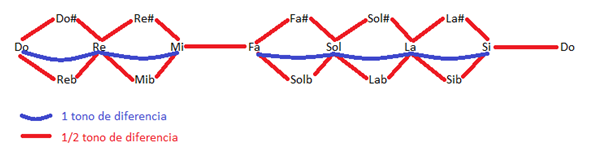
\includegraphics[width=12cm]{tonos.png}}
	\caption{Relacion de tonos y semitonos}
	\label{fig:tonos}
\end{figure}

Como se puede observar entre Mi y Fa existe un semitono, al igual que entre Si y Do.

El pentagrama es un sistema de cinco l�neas y cuatro espacios para escribir m�sica:

\begin{figure}[H]
	\centerline{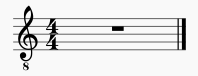
\includegraphics[width=4cm]{pentagrama.png}}
	\caption{Pentagrama}
	\label{fig:pentagrama}
\end{figure}

Este sistema puede tener diferentes elementos dentro de los principales tenemos:

\begin{itemize} [noitemsep]
	\item Clave.
	\item Comp�s.
	\item Armadura. 
	\item Notas.
\end{itemize}

\subsection{Claves musicales}

Las claves musicales se usan para darle nombre y altura a las notas musicales dentro de un pentagrama.

Las claves m�s usadas en la m�sica son: la clave de Sol, la clave de Fa y la clave de Do.

La clave de Sol se usa en instrumentos agudos como la guitarra, viol�n, entre otros. Esta clave normalmente se escribe empezando en la segunda l�nea del pentagrama para formar una especie de G. El hecho de que esta clave se escriba en la segunda l�nea establece que esa l�nea ser� llamada como el nombre de la clave, en este caso Sol:

\begin{figure}[H]
	\centerline{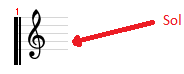
\includegraphics[width=4cm]{clave_sol.png}}
	\caption{Clave de Sol en 2da. Linea}
	\label{fig:clave_sol}
\end{figure}

La clave de Fa es usada en instrumentos m�s graves, tales como el contrabajo, el bajo, etc. Normalmente se escribe empezando en la cuarta l�nea, de tal manera que esta l�nea tomara el nombre de Fa:

\begin{figure}[H]
	\centerline{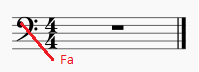
\includegraphics[width=4cm]{clave_fa.png}}
	\caption{Clave de Fa en 4ta. Linea}
	\label{fig:clave_fa}
\end{figure}

La clave de Do es usada com�nmente para las voces, y esta clave se escribe en diferentes l�neas dependiendo del timbre de la voz, para un tenor se usa la clave de Do en 4ta l�nea, mientras que para un soprano normalmente la clave se usa en 3ra o 2da l�nea:

\begin{figure}[H]
	\centerline{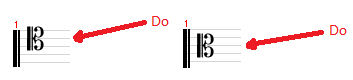
\includegraphics[width=8cm]{clave_do.png}}
	\caption{Clave de Do en 4ta. y 3ra. linea}
	\label{fig:clave_do}
\end{figure}

A partir de estas claves se le puede poner nombre a las diferentes l�neas y espacios del pentagrama, por ejemplo en la clave de sol en segunda l�nea, el pentagrama quedar�a de la siguiente forma:

\begin{figure}[H]
	\centerline{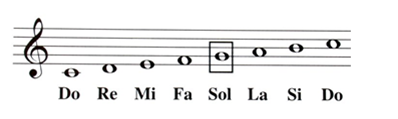
\includegraphics[width=8cm]{notas_clave_sol.png}}
	\caption{Nombre de las notas en un pentagrama con clave de Sol}
	\label{fig:notas_clave_sol}
\end{figure}

\subsection{Compases y tiempo}

El comp�s se puede definir como la unidad m�trica de la m�sica, es la que nos dice que tiempo llevara la canci�n.

Existen una infinidad de compases los cuales podemos clasificar en dos grandes grupos:

\begin{itemize} [noitemsep,nolistsep]
	\item Compases regulares.
	\item Compases irregulares.
\end{itemize}

Los compases regulares est�n regidos por formas regulares las cuales dictan el tiempo, mientras que en los compases irregulares hay que determinar la base de tiempo de forma indirecta.

Cada nota puede tener un valor de tiempo y este valor estar� determinado por el comp�s que se est� utilizando, por ejemplo en un comp�s de 4/4 las figuras musicales tendr�n los siguientes valores:

\begin{table}[H]
	\begin{center}
		\begin{tabular}{|l|l|l|l|}
			\hline
			Nombre & Figura & Silencio & Valor/Pulsos\\
			\hline \hline \hline \hline
			Redonda      & \Ganz & \GaPa & 4 Tiempos \\ \hline
			Blanca       & \Halb & \HaPa & 2 Tiempos \\ \hline
			Negra        & \Vier & \ViPa & 1 Tiempo \\ \hline
			Corchea      & \Acht & \AcPa & $1/2$ Tiempo \\ \hline
			Semicorchea  & \Sech & \SePa & $1/4$ Tiempo \\ \hline
			Fusa         & \Zwdr & \ZwPa & $1/8$ Tiempo \\ \hline
		\end{tabular}
		\caption{Duraci�n de notas musicales.}
		\label{tabla:notes_val}
	\end{center}
\end{table}

Como se puede observar para cada figura musical existe su silencio correspondiente, el cual tendr� el mismo valor solo que este caso no se producir� sonido alguno.

Podemos tener tambi�n los valores relativos de estas notas respecto a otras notas:

\begin{table}[H]
	\begin{center}
		\begin{tabular}{|l|l|l|l|l|l|l|l|}
			\hline
			 &  & \Ganz & \Halb & \Vier & \Acht & \Sech & \Zwdr\\
			\hline \hline \hline \hline \hline
			Redonda      & \Ganz & 1      & 2      & 4     & 8     & 16    & 32 \\ \hline
			Blanca       & \Halb & $1/2$  & 1      & 2     & 4     & 8     & 16 \\ \hline
			Negra        & \Vier & $1/4$  & $1/2$  & 1     & 2     & 4     & 8 \\ \hline
			Corchea      & \Acht & $1/8$  & $1/4$  & $1/2$ & 1     & 2     & 4 \\ \hline
			Semicorchea  & \Sech & $1/16$ & $1/8$  & $1/4$ & $1/2$ & 1     & 2 \\ \hline
			Fusa         & \Zwdr & $1/32$ & $1/16$ & $1/8$ & $1/4$ & $1/2$ & 1 \\ \hline
		\end{tabular}
		\caption{Valor relativo de las notas.}
		\label{tabla:valor_rel}
	\end{center}
\end{table}

De tal manera que en un comp�s tendremos dos datos los cuales se describen a continuaci�n:

\begin{figure}[H]
	\centerline{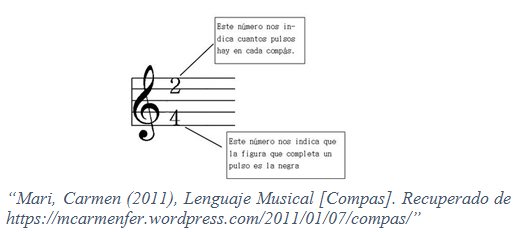
\includegraphics[width=4cm]{compas.png}}
	\caption{Compas}
	\label{fig:compas}
\end{figure}

Se puede ver que este compas tendr� 2 pulsos y el valor de cada pulso ser� de un tiempo de negra, ya que el valor relativo de la negra respecto a la redonda es de $1/4$.

Otro punto a considerar en los compases es que estos tienen tiempos fuertes, semifuertes y d�biles. La cuadratura de una armon�a usa estos tiempos para indicar los cambios que se deben de hacer.

Este es un ejemplo de los tiempos en compases de $4/4$, $3/4$ y $2/4$: 

\begin{figure}[H]
	\centerline{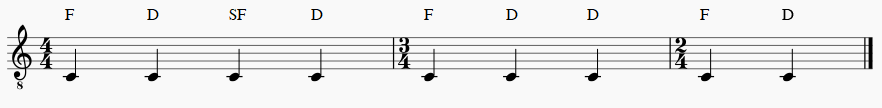
\includegraphics[width=12cm]{tiempos_fd.png}}
	\caption{Tiempos fuertes y d�biles}
	\label{fig:tiempos_fd}
\end{figure}

\subsection{Escalas}

Las escalas son una serie de notas musicales que siguen un orden establecido por intervalos desde una nota base. En el mundo de la m�sica hay una infinidad de escalas pero todas parten de la escala mayor de Do:

\begin{figure}[H]
	\centerline{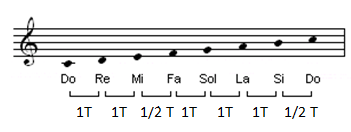
\includegraphics[width=8cm]{escala.png}}
	\caption{Escala de Do Mayor}
	\label{fig:escala}
\end{figure}

En la escala mayor se tiene los siguientes intervalos: tono, tono, semitono, tono, tono, tono, semitono, si esta f�rmula la aplicamos con las otras notas musicales podremos construir todas las escalas mayores.

Por ejemplo la escala de sol mayor quedar�a de la siguiente manera:

\begin{figure}[H]
	\centerline{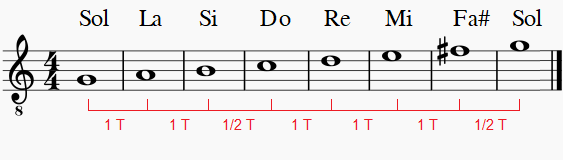
\includegraphics[width=8cm]{escala_sol.png}}
	\caption{Escala de Sol Mayor}
	\label{fig:escala_sol}
\end{figure}

Para poder completar el tono completo de la f�rmula de la escala mayor entre Mi y Fa se tuvo que poner una alteraci�n en la nota de Fa.

La �nica escala mayor que no posee alteraciones es la escala mayor de Do, de ah� en m�s todas las dem�s escalas mayores tendr�n al menos una alteraci�n.

Las escalas menores parten de la escala mayor obteniendo su sexta nota y siguiendo las mismas notas de la escala mayor. Estas escalas menores se les conocen como menores relativas, ya que se basan en una escala mayor para su formaci�n.

Por ejemplo la escala relativa de Do mayor seria La menor y esta escala posee exactamente las mismas notas que la escala mayor solamente que empieza desde la nota de La:

En este caso las notas son: La, Si, Do, Re, Mi, Fa, Sol, La.

\begin{figure}[H]
	\centerline{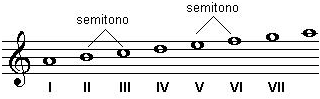
\includegraphics[width=8cm]{escala_la_men.png}}
	\caption{Escala de La menor}
	\label{fig:escala_la_men}
\end{figure}

Esta relatividad puede ser usada con todas las escalas mayores para obtener sus relativas menores.

A pesar que las escalas mayores y menores poseen las mismas notas no deben ser nunca confundidas ya que el sonido final producido es muy diferente, mientras las escalas mayores se usan para canciones se puede decir hasta cierto punto alegres, las escalas menores normalmente acompa�an melod�as melanc�licas, esto no es en todos los casos.

\subsection{Armaduras}

Todas las alteraciones de una escala se pueden juntar al inicio del pentagrama para dar lugar a lo que se conoce como armaduras.

Estas armaduras indicaran que todas las notas que poseen alteraciones las mantendr�n a lo largo de toda la canci�n.

Debido a que las escalas mayores y sus relativas menores poseen las mismas alteraciones comparten tambi�n la misma armadura:

\begin{figure}[H]
	\centerline{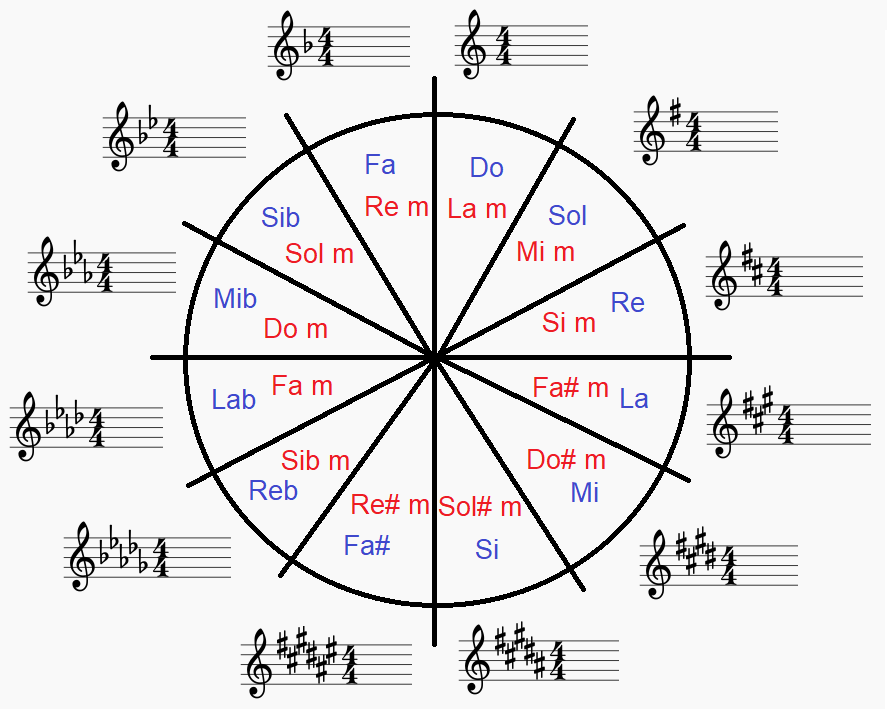
\includegraphics[width=10cm]{armaduras.png}}
	\caption{Armaduras}
	\label{fig:armadura}
\end{figure}

\subsection{Tonalidades}

La tonalidad de una canci�n se basa en la escala base de la canci�n y esta la podemos averiguar viendo la armadura que posee la canci�n, aunque como se vio anteriormente las escalas mayores y sus relativas poseen la misma armadura, as� que antes de definir la tonalidad en base a la armadura tambi�n se debe de hacer un an�lisis de la interacci�n de las notas en la canci�n.

Dentro de las tonalidades tenemos tonalidades mayores y menores, por ejemplo si vemos un pentagrama el cual no posee alteraciones podr�amos asumir que la canci�n esta en Do mayor o en La menor, el siguiente paso ser�a ver la interacci�n de las notas en la canci�n para determinar correctamente la tonalidad.

\subsection{Melod�as y Armon�as}

Una melod�a es una sucesi�n de notas de forma ascendente o descendente que llevan cierta cordura. 

Las melod�as suelen estar formadas por frases y generalmente se repiten a lo largo de una canci�n variando algunas notas intermedias. En este caso se trata de una sucesi�n de notas que no son tocadas al mismo tiempo sino que una nota es tocada despu�s de la otra.

Las armon�as son una conjunci�n de sonidos tocados al mismo tiempo, normalmente la sucesi�n de varios acordes arm�nicos est� ligado directamente con la melod�a de la canci�n.

La armon�a ha cambiado considerablemente desde la �poca de la m�sica barroca hasta la m�sica moderna, anteriormente para generar sistemas arm�nicos se usaban varios instrumentos tocando una nota en espec�fico y la conjunci�n de todos los sonidos daba como resultado la armon�a, actualmente la armon�a es creada a partir de acordes de instrumentos que puedan generar este tipo de condiciones.

Esta es una comparativa para diferenciar entre lo que ser�a una melod�a y una armon�a:

\begin{figure}[H]
	\centerline{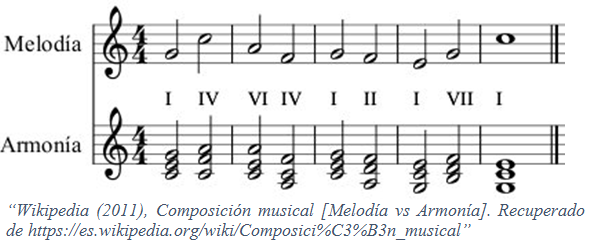
\includegraphics[width=8cm]{melo_armo.png}}
	\caption{Melod�a y Armon�a}
	\label{fig:melo_armo}
\end{figure}

\newpage

\section{Formato MIDI}

MIDI (Interfaz digital de instrumentos musicales) es un est�ndar t�cnico que describe un protocolo, una interfaz digital y conectores para la interoperabilidad entre varios instrumentos musicales electr�nicos, software y dispositivos. \cite{Lear_Coli}

Los archivos MIDI transmiten datos, no sonidos, y estos datos son almacenados en Tracks. Cada archivo MIDI puede tener 1 o mas Tracks.

Los Tracks poseen mensajes de eventos que especifican informaci�n de notas (como tono y velocidad), as� como se�ales de control para par�metros (como volumen, vibrato y se�ales de reloj). Tambien hay eventos que dan informacion acerca del instrumento, clave musical y tiempo. En la figura \ref{fig:formato_midi} se observa la estructura de un archivo MIDI.

\begin{figure}[H]
	\centerline{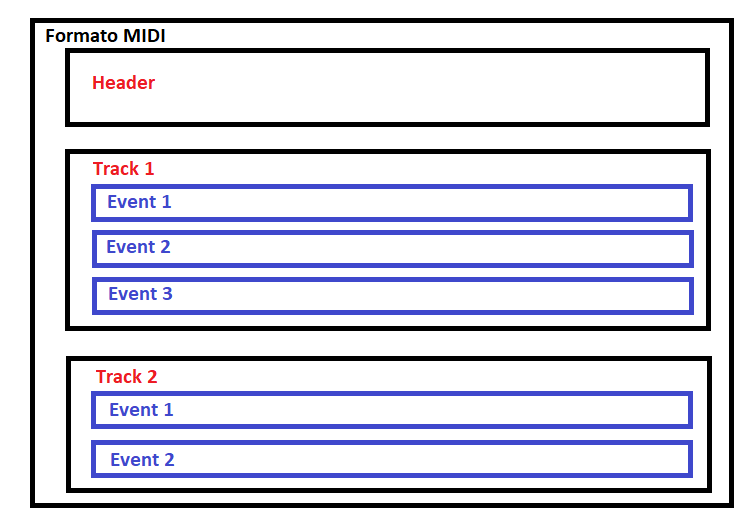
\includegraphics[width=12cm]{formato_midi.png}}
	\caption{Formato MIDI}
	\label{fig:formato_midi}
\end{figure}

Los mensajes MIDI estan estructurados en octetos, por lo que solo pueden existir $2^{3}$ tipos de mensajes diferentes. Cuando se transmiten, a cada octeto se le agrega el bit de paridad con la finalidad de detectar errores en la transmici�n o recepci�n.

En la tabla \ref{tabla:mensajes_midi} se muestran los diferentes eventos que existen y sus parametros:

\begin{table}[H]
	\begin{center}
		\begin{tabular}{|l|l|l|l|}
			\hline
			Mensaje & C�digo & Parametro 1 & Parametro 2\\
			\hline \hline \hline \hline
			Note Off               & 0x8 & Numero de nota        & Velocidad \\ \hline
			Note On                & 0x9 & Numero de nota        & Velocidad \\ \hline
			Polyphonic aftertouch  & 0xA & Numero de nota        & Presi�n \\ \hline
			Control Change         & 0xB & Numero de controlador & Datos \\ \hline
			Program Change         & 0xC & Numero de programa    & - \\ \hline
			Channel aftertouch     & 0xD & Presion               & - \\ \hline
			Pitch wheel            & 0xE & LSByte                & MSByte \\ \hline
			System Message         & 0xF & -                     & - \\ \hline
		\end{tabular}
		\caption{Mensajes MIDI.}
		\label{tabla:mensajes_midi}
	\end{center}
\end{table}

Cada uno de los mensajes se describen a continuaci�n \cite{Lear_Coli}\cite{sergi_audio}:

\begin{itemize}
	\item \textbf{Note on.-} Este mensaje le indica al dispositivo, que debe iniciar una nota. Indica que una nota debe ser reproducida. Contiene la informaci�n de estado (n�mero de canal, especificado por un entero dentro de [0 15] y dos valores de datos: un n�mero de nota MIDI (el tono de la nota, un entero dentro de [0 127]) y una velocidad (que indica c�mo la nota es reproducida, un entero dentro de [0 127]). Un ejemplo es ''Note on, 0, 60, 50'' que interpreta como: en el canal 1, comienza a reproducir un C medio con una velocidad de 50.
	\item \textbf{Note off.-} Indica que una nota termina. En esa situaci�n, la velocidad indica qu� tan r�pido se libera la nota. Un ejemplo es ''Note off, 0, 60, 20'' que interpreta como: en el canal 1, deja de reproducir un C medio con una velocidad de 20. 
	\item \textbf{Polyphonic aftertouch.-} Algunos teclados de alta gama son capaces de detectar de forma permanente (decenas de veces por segundo) los cambios en la presi�n ejercida sobre cada una de sus teclas. En este	caso, siempre que se produzca alg�n cambio, env�an este mensaje.
	\item \textbf{Control Change.-} Este mensaje engloba 128 posibles mensajes de	control diferentes Todos ellos afectan de alguna forma a la calidad del sonido; existen controles para modificar el volumen, la modulaci�n, la reverberaci�n, etc. 
	\item \textbf{Program Change.-} Evento para designar los diferentes sonidos disponibles en un sintetizador (instrumentos, efectos sonoros, etc.). 
	\item \textbf{Channel aftertouch.-} Este mensaje es parecido al Polyphonic aftertouch con la diferencia de que en lugar de enviar un mensaje de presi�n por cada nota, se envia uno por cada canal.
	\item \textbf{Pitch wheel.-} la inmensa mayor�a de teclados disponen a la izquierda, de
	dos peque�as ruedas giratorias. Una de ellas (la que vuelve autom�ticamente a su posici�n
	central), se utiliza para desafinar ligeramente el sonido. Cuando la rueda gira, el teclado env�a
	estos mensajes de forma ?continua? (decenas de veces por segundo).
	\item \textbf{System Message.-} Estos mensajes se comportan de forma diferente a todos los anteriores, ya que los cuatro bits restantes no indican un n�mero de canal, y por ello, afectan globalmente al comportamiento de los dispositivos que los reciban. Estos cuatro bits restantes, definen de hecho diecis�is mensajes diferentes, que se reparten en tres grupos: los mensajes comunes de sistema, los 	mensajes de sistema de tiempo real y los mensajes de sistema exclusivo. 
\end{itemize}

En la siguiente tabla \ref{tabla:n_notas_midi} se puede observar los valores de las notas y a que octava pertenecen:

\begin{table}[H]
	\begin{center}
		\begin{tabular}{|l|l|l|l|l|l|l|l|l|l|l|l|l|}
			\hline
			Octava & C & C\# & D & D\# & E & F & F\# & G & G\# & A & A\# & B \\
			\hline \hline \hline \hline \hline \hline \hline \hline \hline \hline \hline \hline \hline
			-1 & 0   & 1   & 2   & 3   & 4   & 5   & 6   & 7   & 8   & 9   & 10  & 11  \\ \hline
			0  & 12  & 13  & 14  & 15  & 16  & 17  & 18  & 19  & 20  & 21  & 22  & 23  \\ \hline
			1  & 24  & 25  & 26  & 27  & 28  & 29  & 30  & 31  & 32  & 33  & 34  & 35  \\ \hline
			2  & 36  & 37  & 38  & 39  & 40  & 41  & 42  & 43  & 44  & 45  & 46  & 47  \\ \hline
			3  & 48  & 49  & 50  & 51  & 52  & 53  & 54  & 55  & 56  & 57  & 58  & 59  \\ \hline
			4  & 60  & 61  & 62  & 63  & 64  & 65  & 66  & 67  & 68  & 69  & 70  & 71  \\ \hline
			5  & 72  & 73  & 74  & 75  & 76  & 77  & 78  & 79  & 80  & 81  & 82  & 83  \\ \hline
			6  & 84  & 85  & 86  & 87  & 88  & 89  & 90  & 91  & 92  & 93  & 94  & 95  \\ \hline
			7  & 96  & 97  & 98  & 99  & 100 & 101 & 102 & 103 & 104 & 105 & 106 & 107 \\ \hline
			8  & 108 & 109 & 110 & 111 & 112 & 113 & 114 & 115 & 116 & 117 & 118 & 119 \\ \hline
			9  & 120 & 121 & 122 & 123 & 124 & 125 & 126 & 127 &     &     &     &     \\ \hline
		\end{tabular}
		\caption{Numero de nota en formato MIDI.}
		\label{tabla:n_notas_midi}
	\end{center}
\end{table}

Cada evento de nota est� realmente incrustado en un fragmento de pista, una estructura de datos que contiene un valor de tiempo delta que especifica la informaci�n de temporizaci�n y el evento en s�. Un valor de tiempo delta representa la posici�n de tiempo, como un valor absoluto, del evento y podr�a representar:

\begin{itemize}
	\item \textbf{Metrical time.-} Representa el numero de pulsos desde el comienzo. Una referencia llamada divisi�n y es definida en el encabezado del archivo, especificando cuantos pulsos por nota de cuarto.
	\item \textbf{time-code-based time.-} Representa el tiempo relacionado con horas, minutos y segundos de la canci�n. 
\end{itemize}

Un ejemplo de un extracto de un archivo MIDI y su partitura correspondiente es mostrado en las siguientes figuras \ref{fig:extract_midi} \ref{fig:repres_midi}.

\begin{figure}[H]
	\centerline{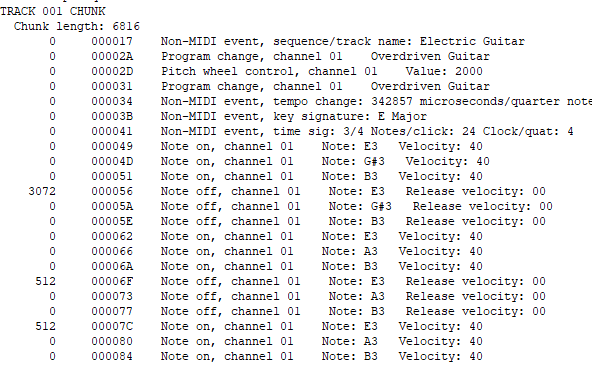
\includegraphics[width=12cm]{eventos_midi.png}}
	\caption{Extracto de un formato MIDI}
	\label{fig:extract_midi}
\end{figure}

\begin{figure}[H]
	\centerline{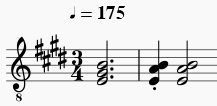
\includegraphics[width=6cm]{repres_midi.png}}
	\caption{Partitura correspondiente al extracto MIDI}
	\label{fig:repres_midi}
\end{figure}

Dentro del formato MIDI se pueden representar en cada track un instrumento diferente, para realizar esto se utiliza el evento "Program Change", el cual dependiendo de su valor, sera el instrumento a reproducir.

\begin{table}[H]
	\begin{center}
		\resizebox{\textwidth}{!}{%
		\begin{tabular}{|l|l|l|l|l|l|l|l|}
			\hline
			PC & Instrumento & PC & Instrumento & PC & Instrumento & PC & Instrumento\\
			\hline \hline \hline \hline \hline \hline \hline \hline
			1    &    Acoustic Grand Piano   &   9    &    Celesta            &   17   &    Drawbar Organ         &   25   &    Acoustic Guitar (nylon) \\ \hline
			2    &    Bright Acoustic Piano  &   10   &    Glockenspiel       &   18   &    Percussive Organ      &   26   &    Acoustic Guitar (steel) \\ \hline
			3    &    Electric Grand Piano   &   11   &    Music Box          &   19   &    Rock Organ            &   27   &    Electric Guitar (jazz) \\ \hline
			4    &    Honky-tonk Piano       &   12   &    Vibraphone         &   20   &    Church Organ          &   28   &    Electric Guitar (clean) \\ \hline
			5    &    Electric Piano 1       &   13   &    Marimba            &   21   &    Reed Organ            &   29   &    Electric Guitar (muted) \\ \hline
			6    &    Electric Piano 2       &   14   &    Xylophone          &   22   &    Accordion             &   30   &    Overdriven Guitar \\ \hline
			7    &    Harpsichord            &   15   &    Tubular Bells      &   23   &    Harmonica             &   31   &    Distortion Guitar \\ \hline
			8    &    Clavi                  &   16   &    Dulcimer           &   24   &    Tango Accordion       &   32   &    Guitar harmonics \\ \hline
			\hline \hline \hline \hline \hline \hline \hline \hline
			33   &    Acoustic Bass          &   41   &    Violin             &   49   &    String Ensemble 1     &   57   &    Trumpet \\ \hline
			34   &    Electric Bass (finger) &   42   &    Viola              &   50   &    String Ensemble 2     &   58   &    Trombone \\ \hline
			35   &    Electric Bass (pick)   &   43   &    Cello              &   51   &    SynthStrings 1        &   59   &    Tuba \\ \hline
			36   &    Fretless Bass          &   44   &    Contrabass         &   52   &    SynthStrings 2        &   60   &    Muted Trumpet \\ \hline
			37   &    Slap Bass 1            &   45   &    Tremolo Strings    &   53   &    Choir Aahs            &   61   &    French Horn \\ \hline
			38   &    Slap Bass 2            &   46   &    Pizzicato Strings  &   54   &    Voice Oohs            &   62   &    Brass Section \\ \hline
			39   &    Synth Bass 1           &   47   &    Orchestral Harp    &   55   &    Synth Voice           &   63   &    SynthBrass 1 \\ \hline
			40   &    Synth Bass 2           &   48   &    Timpani            &   56   &    Orchestra Hit         &   64   &    SynthBrass 2 \\ \hline
			\hline \hline \hline \hline \hline \hline \hline \hline
			65   &    Soprano Sax            &   73   &    Piccolo            &   81   &    Lead 1 (square)       &   89   &    Pad 1 (new age) \\ \hline
			66   &    Alto Sax               &   74   &    Flute              &   82   &    Lead 2 (sawtooth)     &   90   &    Pad 2 (warm) \\ \hline
			67   &    Tenor Sax              &   75   &    Recorder           &   83   &    Lead 3 (calliope)     &   91   &    Pad 3 (polysynth) \\ \hline
			68   &    Baritone Sax           &   76   &    Pan Flute          &   84   &    Lead 4 (chiff)        &   92   &    Pad 4 (choir) \\ \hline
			69   &    Oboe                   &   77   &    Blown Bottle       &   85   &    Lead 5 (charang)      &   93   &    Pad 5 (bowed) \\ \hline
			70   &    English Horn           &   78   &    Shakuhachi         &   86   &    Lead 6 (voice)        &   94   &    Pad 6 (metallic) \\ \hline
			71   &    Bassoon                &   79   &    Whistle            &   87   &    Lead 7 (fifths)       &   95   &    Pad 7 (halo) \\ \hline
			72   &    Clarinet               &   80   &    Ocarina            &   88   &    Lead 8 (bass + lead)  &   96   &    Pad 8 (sweep) \\ \hline
			\hline \hline \hline \hline \hline \hline \hline \hline
			97   &    FX 1 (rain)            &   105  &    Sitar              &   113  &    Tinkle Bell           &   121  &    Guitar Fret Noise \\ \hline
			98   &    FX 2 (soundtrack)      &   106  &    Banjo              &   114  &    Agogo                 &   122  &    Breath Noise \\ \hline
			99   &    FX 3 (crystal)         &   107  &    Shamisen           &   115  &    Steel Drums           &   123  &    Seashore \\ \hline
			100  &    FX 4 (atmosphere)      &   108  &    Koto               &   116  &    Woodblock             &   124  &    Bird Tweet \\ \hline
			101  &    FX 5 (brightness)      &   109  &    Kalimba            &   117  &    Taiko Drum            &   125  &    Telephone Ring \\ \hline
			102  &    FX 6 (goblins)         &   110  &    Bag pipe           &   118  &    Melodic Tom           &   126  &    Helicopter \\ \hline
			103  &    FX 7 (echoes)          &   111  &    Fiddle             &   119  &    Synth Drum            &   127  &    Applause \\ \hline
			104  &    FX 8 (sci-fi)          &   112  &    Shanai             &   120  &    Reverse Cymbal        &   128  &    Gunshot \\ \hline
		\end{tabular}}
		\caption{Instrumentos en formato MIDI.}
		\label{tabla:instr_midi}
	\end{center}
\end{table} 

Los instrumentos de percusi�n no usan este evento, en lugar de eso usan el canal 10 para transmitir los datos.

\newpage

\section{Algoritmo Krumhansl-Schmuckler}

Este algoritmo es usado para determinar o asignar la tonalidad mas apropiada a una serie de notas musicales. Fue dise�ado y desarrollado por Carol L. Krumhansl y Mark A. Schmuckler.

Para determinar cual es la tonalidad mas apropiada, el algoritmo hace uso del coeficiente de correlacion de Pearson:

\begin{equation}
R = \frac{\displaystyle\sum_{i=1}^{n}(x_i - \bar{x})(y_i - \bar{y})}{\sqrt{\displaystyle\sum_{i=1}^{n}(x_i - \bar{x})^{2}\displaystyle\sum_{i=1}^{n}(y_i - \bar{y})^{2}}}
\label{ec:coeficiente}
\end{equation}

El cual dado un conjunto de datos $(x, y)$ determina un valor entre $[-1, 1]$ el cual indica si el conjunto de datos $x$ tiene relacion con el conjunto de datos $y$:

\begin{itemize}
	\item \textbf{0 : } Indica que no hay relaci�n lineal entre $x$ y $y$
	\item \textbf{1 : } Indica que hay una correlaci�n perfecta positiva, si $x$ crece $y$ tambi�n.
	\item \textbf{-1 : } Indica que hay una correlaci�n perfecta negativa, si $x$ crece $y$ decrece.
\end{itemize}

En el algoritmo para encontrar la tonalidad, una de las cordenadas representa un perfil de una tonalidad mayor (tabla \ref{tabla:per_ton_may}) o una tonalidad menor (tabla \ref{tabla:per_ton_men}). 

\begin{table}[H]
	\begin{center}
		\begin{tabular}{|l|l|l|l|l|l|l|l|l|l|l|l|}
			\hline
			Do & Do\# & Re & Re\# & Mi & Fa & Fa\# & Sol & Sol\# & La & La\# & Si \\ \hline
			6.35 & 2.23  & 3.48  & 2.33 & 4.38 & 4.09 & 2.52 & 5.19 & 2.39 & 3.66 & 2.29 & 2.88  \\ \hline
		\end{tabular}
		\caption{Perfil de tonalidades mayores.}
		\label{tabla:per_ton_may}
	\end{center}
\end{table}

\begin{table}[H]
	\begin{center}
		\begin{tabular}{|l|l|l|l|l|l|l|l|l|l|l|l|}
			\hline
			la & la\# & si & do & do\# & re & re\# & mi & fa & fa\# & sol & sol\# \\ \hline
			6.33 & 2.68 & 3.52  & 5.38 & 2.60 & 3.53 & 2.54 & 4.75 & 3.98 & 2.69 & 3.34 & 3.17  \\ \hline
		\end{tabular}
		\caption{Perfil de tonalidades menores.}
		\label{tabla:per_ton_men}
	\end{center}
\end{table}

El otro valor de las coordenadas es el total de duraci�n de cada nota en la pieza musical siendo analizada. En la tabla \ref{tabla:dur_ejemplo} se observa un ejemplo de los valores de una canci�n:

\begin{table}[H]
	\begin{center}
		\begin{tabular}{|l|l|l|l|l|l|l|l|l|l|l|l|}
			\hline
			C & C\# & D & D\# & E & F & F\# & G & G\# & A & A\# & B \\ \hline
			432 & 231  & 0  & 405 & 12 & 316 & 4 & 126 & 612 & 0 & 191 & 1  \\ \hline
		\end{tabular}
		\caption{Ejemplo de duraci�n de notas en una canci�n.}
		\label{tabla:dur_ejemplo}
	\end{center}
\end{table}

El algoritmo calcula el coeficiente de correlaci�n para todas las posibles tonalidades mayores y menores. En las tablas \ref{tabla:cor_do_may} y \ref{tabla:cor_re_may} se muestra un ejemplo de como se empiezan a relacionar los datos de la cancion con los perfiles de las tonalidades:

\begin{table}[H]
	\begin{center}
		\begin{tabular}{|l|l|}
			\hline
			(Do, C)      &  (6.35, 432)  \\ \hline
			(Do\#, C\#)  &  (2.23, 231)  \\ \hline
			(Re, D)      &  (3.48, 0)  \\ \hline
			(Re\#, D\#)  &  (2.33, 405)  \\ \hline
			(Mi, E)      &  (4.38, 12)  \\ \hline
			(Fa, F)      &  (4.09, 316)  \\ \hline
			(Fa\#, F\#)  &  (2.52, 4)  \\ \hline
			(Sol, G)     &  (5.19, 126)  \\ \hline
			(Sol\#, G\#) &  (2.39, 612)  \\ \hline
			(La, A)      &  (3.66, 0)  \\ \hline
			(La\#, A\#)  &  (2.29, 191)  \\ \hline
			(Si, B)      &  (2.88, 1)  \\ \hline
		\end{tabular}
		\caption{Correlaci�n de Do Mayor.}
		\label{tabla:cor_do_may}
	\end{center}
\end{table} 

En el caso de la tonalidad de Do Mayor obtenemos un coeficiente de correlaci�n de $R=0.00009$, lo que significa que no hay probabilidad de que esta sea la tonalidad adecuada para la canci�n.

Si se grafican los puntos de las coordenadas $(x, y)$ para esta tonalidad se vera que los puntos estan demasiados dispersos entre si, por lo tanto no podemos encontrar una linea recta que prediga la posici�n de nuevos puntos.

Ahora vamos a analizar que pasa con la tonalidad de Re Mayor.

\begin{table}[H]
	\begin{center}
		\begin{tabular}{|l|l|}
			\hline
			(Do, D)      &  (6.35, 0)  \\ \hline
			(Do\#, D\#)  &  (2.23, 405)  \\ \hline
			(Re, E)      &  (3.48, 12)  \\ \hline
			(Re\#, F)    &  (2.33, 316)  \\ \hline
			(Mi, F\#)    &  (4.38, 4)  \\ \hline
			(Fa, G)      &  (4.09, 126)  \\ \hline
			(Fa\#, G\#)  &  (2.52, 612)  \\ \hline
			(Sol, A)     &  (5.19, 0)  \\ \hline
			(Sol\#, A\#) &  (2.39, 191)  \\ \hline
			(La, B)      &  (3.66, 1)  \\ \hline
			(La\#, C)    &  (2.29, 432)  \\ \hline
			(Si, C\#)    &  (2.88, 231)  \\ \hline
		\end{tabular}
		\caption{Correlaci�n de Re Mayor.}
		\label{tabla:cor_re_may}
	\end{center}
\end{table} 

En este caso los puntos no se encuentran tan dispersos, por lo que obtenemos un coeficiente de correlaci�n de $R=-0.74$, lo que significa que existe una gran correlaci�n negativa.

Si se realiza este mismo ejercicio con todas las posibles tonalidades obtendremos que la tonalidad que obtuvo mayor correlaci�n es Sol\# Mayor con un coeficiente de $R=0.97$, por lo tanto esta seria la tonalidad mas adecuada de la pieza.

Este algoritmo regresa una lista ordenada de todos los valores posibles y su coeficiente de correlaci�n, donde el primer elemento es el que mayor correlaci�n contiene, y as� sucesivamente para los siguientes elementos
%IMD PNA http://na.support.keysight.com/pna/help/latest/Applications/Swept_IMD_Configure_External_Source_and_Combiner.htm
\chapter{Conclusiones}

%%-----------------------------------------------------------------------







% se incluye la bibliograf�a en su respectivo .bib y con el estilo deseado

\bibliography{bibliografia}
\bibliographystyle{IEEEtran}
\nocite{*}

\backmatter
\end{document}
